% \documentclass[8pt,xcolor=pdftex,table,handout]{beamer}

\documentclass[8pt,xcolor=pdftex,table]{beamer}
\include{preambule_beamer}

\usepackage{listings}

% \usepackage{amsmath}
% \usepackage{unicode-math}
% \setmathfont{Fira Math}


% \usepackage{animate}

% ------------------------------------------- %

\graphicspath{{Figures/} {Figures/Logos/} {../Figures/}}
% \graphicspath{{../Figures/} {../Figures/Logos/}}

\title[]{\vspace{22mm}Formation \alert{Ingénieur Machine Learning}\\\vspace{6mm}Projet:\\\alert{Développez une preuve de concept}}
\date[]{9 Août 2023\\\vspace{18mm}\\\tit{thomas.durandtexte@protonmail.com}}


\titlegraphic{\hfill
\def\arraystretch{.1}%  1 is the default, change whatever you need
	\begin{tabular}{ >{\centering}m{7mm} m{39mm} }
		
\includegraphics[height=7mm]{Logo_OpenClassrooms.png }
		&
		\Large{\textbf{OPENCLASSROOMS}}
	\end{tabular}
}

% \definecolor{clrData}{rgb}{0.9,0.5,0}

\tikzstyle{box}=[draw, rounded corners,anchor=center,text centered,text=white]
% \tikzstyle{diagram0}=[box, text width=22mm, minimum height=12mm]
% \tikzstyle{dataset}=[box,diagram0, fill=blue]
% \tikzstyle{filtrage}=[box,diagram0, fill=red!80]
% \tikzstyle{doublons}=[box,diagram0, fill=magenta!80]
% \tikzstyle{datavoisins}=[box,diagram0, fill=cyan!80]
% \tikzstyle{outliers}=[box,diagram0, fill=magenta!80]

% \includeonlyframes{ArchitectureGenerale}



\begin{document}
% ------------------------------------------- %

\begin{frame}
	\titlepage{}
\end{frame}


\section{CONTEXTE}


\begin{frame}[t, label=contexte]
	\vspace{0mm}
	\centering
	\vfill
	\begin{tikzpicture}
		\linespread{1}% <--- locally defined vertical line spacing in nodes
		\drawBorder
		\nodePageNumber

		\onlystyle<2->{removed}{myShaded}
		\onlystyle<4->{shaded1}{myShaded}
		\node[removed, text centered] at (0.5\txw,80mm)
			{Corrélation d'Images Numériques} ;

		% \visible<2->{
		% \node[box] at (0.5\txw, 60mm) (I)
		% 	{Images de chiens \alert{à trier}} ;
		% }
		% \visible<3->{
		% 	\node[box] at (0.5\txw, 40mm) (DL)
		% 		{Modèle \alert{Deep Learning}} ;
		% 	\draw[myarrow] (I) -- (DL) ;
		% }

		% \visible<4->{
		% 	\node[box] at (0.5\txw, 20mm) (I2)
		% 		{Images de chiens \alert{triées}} ;
		% 	\draw[myarrow] (DL) -- (I2) ;
		% }
		\visible<2->{
		\begin{scope}[xshift=35mm, yshift=36mm]
			\node {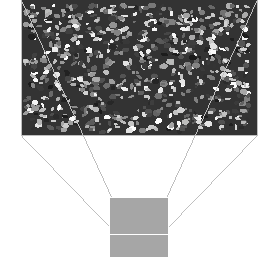
\includegraphics[width=60mm]{camera.pdf}} ;
			\node at (-13mm, -23mm) {Caméra} ;
			\node at (3mm, 32mm) {Surface mesurée} ;
		\end{scope}
		}

		\begin{scope}[xshift=85mm, yshift=65mm]
			\node<3->[shaded1, text centered, text width=30mm] {Méthode de mesure de :} ;

			\node<4->[box] at (0,-15mm) {Formes} ;
			\node<5->[box] at (0,-30mm) {Déplacements} ;
			\node<6->[box] at (0,-45mm) {Déformations} ;
		\end{scope}
	\end{tikzpicture}
	\vfill
\end{frame}



\begin{frame}[t, label=contexte2]
	\vspace{0mm}
	\centering
	\vfill
	\begin{tikzpicture}
		\linespread{1}% <--- locally defined vertical line spacing in nodes
		\drawBorder
		\nodePageNumber

		\onlystyle<2->{removed}{myShaded}
		\onlystyle<4->{shaded1}{myShaded}
		\node[removed, text centered] at (0.5\txw,80mm)
			{Corrélation d'Images Numériques : principe} ;

			\begin{scope}[xshift=\midX-40mm, yshift=\midY-25mm, scale=2, line width=1.5]
				\visible<2->{
					\node at (-0.05, -0.15) {} ;
					\node at (4.05, 2.05) {} ;
					% \draw[line width=1] (-1, 0) -- (1, 0) -- (0,0) -- (0, 2) -- (0, -2) ;
					\draw[myarrow, line width=2] (-0.007, -0.1) -- ++ (4, 0) ;
					\draw[myarrow, line width=2] (0, -0.1) -- ++ (0, 2.15) ;
					\node at (3.9, 0.01) {x} ;
					\node at (0.25, 1.9) {I(x)} ;
				}

				\visible<4->{
					\draw[color=black!40] (1.5,1) -- ++(0.55,0) ;
					\node[color=black!40, text centered] at (1.9, 1.15) {$\pmb{\Delta x}$} ;
					\draw[color=black!40] (1.5,1) -- ++(0,0-0.55) ;
					\node[color=black!40, text centered] at (1.65, 0.8) {$\pmb{\Delta I}$} ;
				}

				\draw<2-> (0, 0) -- ++ (0.5, 0) -- ++(2, 2) -- ++(1, 0) ;
				\node<2-> (fx) at (1.5,1.5) {F(x)} ;

				\draw<3->[red] (0.55, 0) -- ++ (0.5, 0) -- ++(2, 2) -- ++(0.5, 0) ;
				\node<3->[color=red] (gx) at (2.7,1.2) {G(x)} ;

				\node<5->[draw, rounded corners, text centered]
					at (3, 0.5) {$\pmb{\Delta x = -\dfrac{\Delta I}{\partial F(x)/\partial x}}$ } ;
			\end{scope}
	\end{tikzpicture}
	\vfill
\end{frame}


\begin{frame}[t, label=contexte3]
	\vspace{0mm}
	\centering
	\vfill
	\begin{tikzpicture}
		\linespread{1}% <--- locally defined vertical line spacing in nodes
		\drawBorder
		\nodePageNumber

		\onlystyle<2->{removed}{myShaded}
		\onlystyle<4->{shaded1}{myShaded}
		\node[removed, text centered] at (0.5\txw,80mm)
			{Corrélation d'Images Numériques : processus itératif} ;

		\begin{scope}[yshift=62mm]
			\node<2-> at (\midX-20mm,0) {image de référérence} ;
			\node<2-> at (\midX+20mm,0) {image déformée} ;
		\end{scope}
		\node<2> at (\midX,40mm) {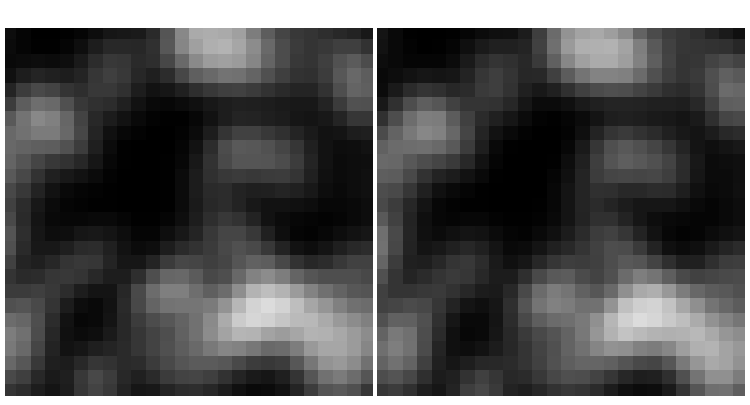
\includegraphics[width=80mm]{dic/dic_example-0.pdf}} ;%
		\node<3> at (\midX,40mm) {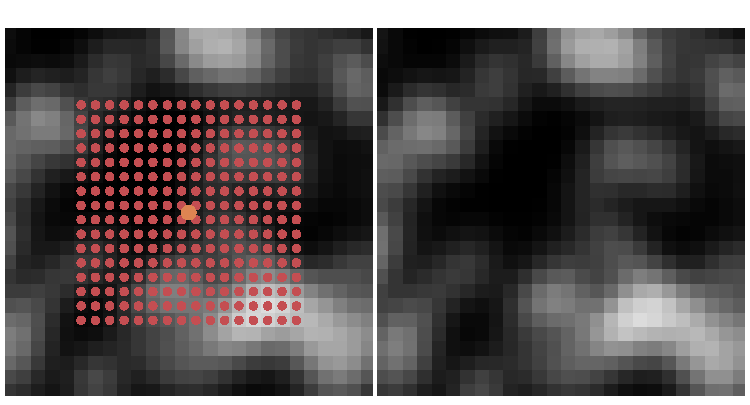
\includegraphics[width=80mm]{dic/dic_example-1.pdf}} ;%
		\node<3->[red] at (20mm, 15mm) {\textit{subset}} ;
		\node<4> at (\midX,40mm) {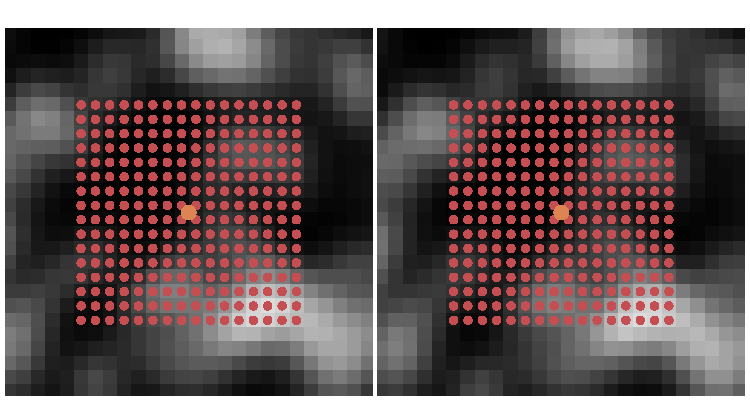
\includegraphics[width=80mm]{dic/dic_example-2.pdf}} ;%

		\node<5> at (\midX,40mm) {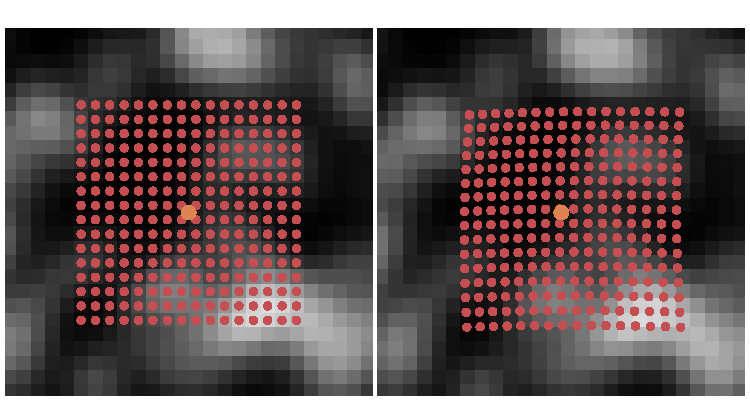
\includegraphics[width=80mm]{dic/dic_example-3.pdf}} ;%
		\node<6> at (\midX,40mm) {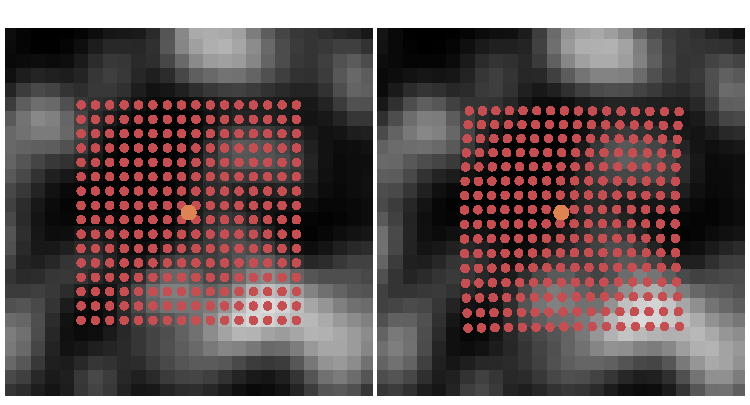
\includegraphics[width=80mm]{dic/dic_example-4.pdf}} ;%
		\node<7> at (\midX,40mm) {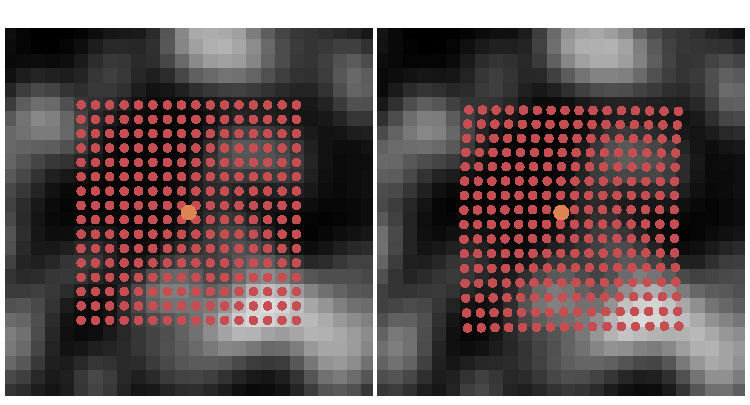
\includegraphics[width=80mm]{dic/dic_example-5.pdf}} ;%
		\node<8> at (\midX,40mm) {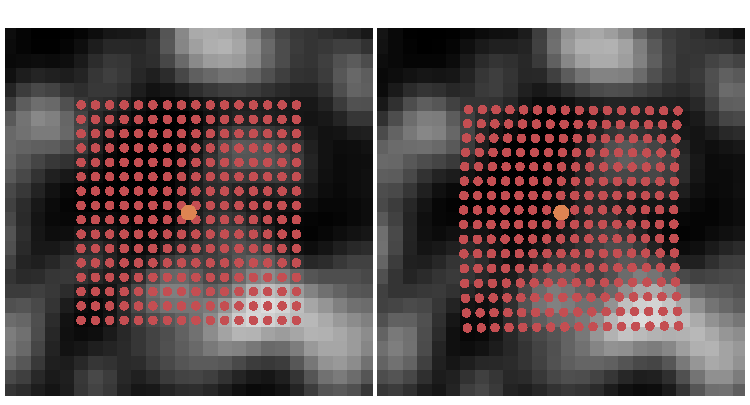
\includegraphics[width=80mm]{dic/dic_example-6.pdf}} ;%
		\node<9> at (\midX,40mm) {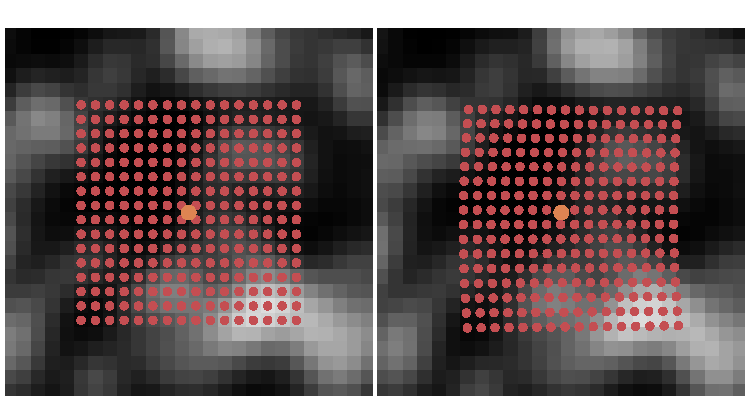
\includegraphics[width=80mm]{dic/dic_example-7.pdf}} ;%
		\node<10> at (\midX,40mm) {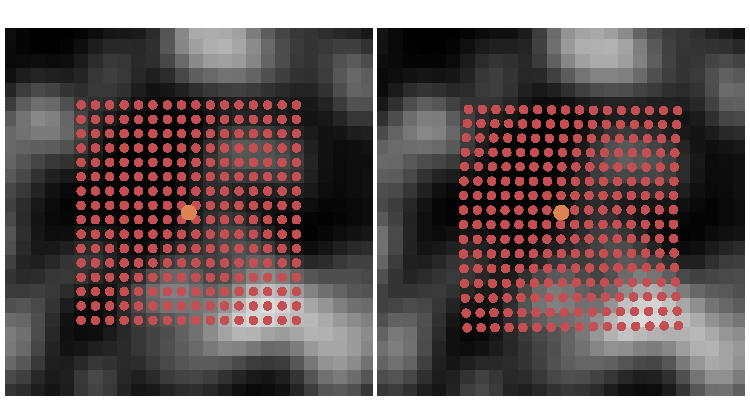
\includegraphics[width=80mm]{dic/dic_example-8.pdf}} ;%
		\node<11> at (\midX,40mm) {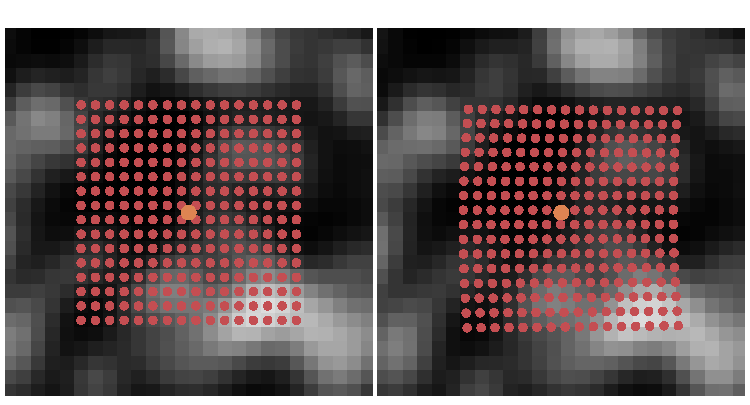
\includegraphics[width=80mm]{dic/dic_example-9.pdf}} ;%
		\node<12> at (\midX,40mm) {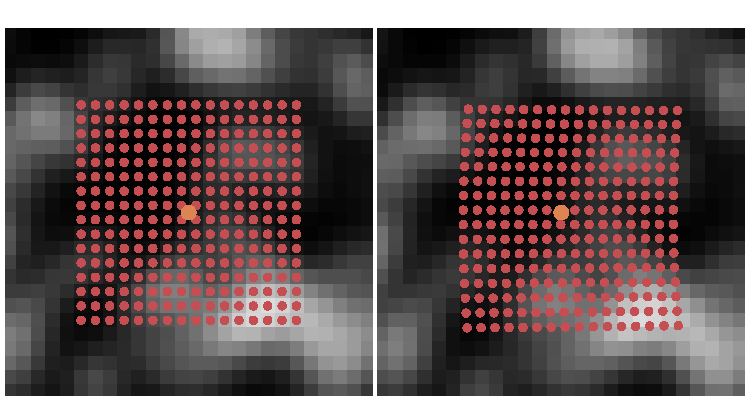
\includegraphics[width=80mm]{dic/dic_example-10.pdf}} ;%
		\begin{scope}[xshift=\midX, yshift=15mm]
			\node<3-4> {Initialisation} ;
			\node<5> {Itération 1} ;
			\node<6> {Itération 2} ;
			\node<7> {Itération 3} ;
			\node<8> {Itération 4} ;
			\node<9> {Itération 5} ;
			\node<10> {Itération 6} ;
			\node<11> {Itération 7} ;
			\node<12> {Itération 8} ;
		\end{scope}
	\end{tikzpicture}
	\vfill
\end{frame}


\begin{frame}[t, label=objectifs]
	\vspace{0mm}
	\centering
	\vfill
	\begin{tikzpicture}
		\linespread{1}% <--- locally defined vertical line spacing in nodes
		\drawBorder
		\nodePageNumber

		\onlystyle<2->{shd1}{myShaded}
		\onlystyle<6->{shd2}{myShaded}
		% \onlystyle<4->{shd3}{myShaded}
		% \onlystyle<5->{shd4}{myShaded}
		% \onlystyle<6->{shd5}{myShaded}
		% \onlystyle<7->{shd6}{myShaded}
		\node[shd1] at (\midX,75mm) {Objectifs} ;
		\node<5->[shd2] at (\midX,40mm) {Finalité} ;

		\begin{scope}[xshift=\midX, yshift=60mm]
			\node<2->[box] at (-35mm,0) {\alert{Générer} un dataset} ;
			\node<3->[box, text width=35mm] at (0mm,0) {\alert{Construire} et \alert{optimiser} un réseau de neuronnes} ;
			\node<4->[box, text width=20mm] at (35mm,0) {\alert{Entrainer} le réseau de neuronnes} ;
		\end{scope}

		\begin{scope}[xshift=\midX, yshift=25mm]
			\node<6->[box, text width=25mm] at (-20mm,0) {\alert{Limiter} les temps de calcul} ;
			% \node<3->[box, text width=35mm] at (0mm,0) {\alert{Construire} et \alert{optimiser} un réseau de neuronnes} ;
			\node<7->[box, text width=25mm] at (20mm,0) {\alert{Améliorer} la précision de mesure} ;
		\end{scope}
	\end{tikzpicture}
	\vfill
\end{frame}


\section{GÉNÉRATION DES IMAGE}
\begin{frame}[t, label=GenImages]
	\vspace{0mm}
	\centering
	\vfill
	\begin{tikzpicture}
		\linespread{1}% <--- locally defined vertical line spacing in nodes
		\drawBorder
		\nodePageNumber

		\onlystyle<2->{shd1}{myShaded}
		% \onlystyle<3->{shd2}{myShaded}
		% \onlystyle<4->{shd3}{myShaded}
		% \onlystyle<5->{shd4}{myShaded}
		% \onlystyle<6->{shd5}{myShaded}
		% \onlystyle<7->{shd6}{myShaded}
		\node[shd1] at (\midX,80mm) {Génération des images~: protocole} ;

		\begin{scope}[xshift=\midX-25mm, yshift=\midY+10mm]
			\node (A0) at (0, 0) {} ;
			\node (B0) at (40mm, 0) {} ;
			\node (Ca0) at (0, -20mm) {} ;
			\node (Cb0) at (40mm, -20mm) {} ;

			\node<2->[box, text width=38mm] (A) {Génération d'une\\image de mouchetis};
			\node<3->[box, text width=38mm, minimum height=8.3mm, right=of A] (B)
				{Transformations} ;
			\node<4->[box, text width=38mm, below=of A] (Ca) {Déformation} ;
			\node<6->[box, text width=38mm, below right=of A] (Cb) {Re-échantillonnage} ;
			\node<5->[box, text width=38mm, below=of Ca] (Da) {Image de référence} ;
			\node<7->[box, text width=38mm, below=of Cb] (Db) {Image déformée} ;

			\draw<3->[myarrow] (A) -- (B) ;
			\draw<4->[myarrow] (B) -- ++ (0, -9mm) -| (Ca) ;
			\draw<6->[myarrow] (B) -- (Cb) ;
			\draw<5->[myarrow] (Ca) -- (Da) ;
			\draw<7->[myarrow] (Cb) -- (Db) ;
		\end{scope}

	\end{tikzpicture}
	\vfill
\end{frame}


\begin{frame}[t, label=GenSpeckles]
	\vspace{0mm}
	\centering
	\vfill
	\begin{tikzpicture}
		\linespread{1}% <--- locally defined vertical line spacing in nodes
		\drawBorder
		\nodePageNumber

		\onlystyle<2->{shd1}{myShaded}
		% \onlystyle<3->{shd2}{myShaded}
		% \onlystyle<4->{shd3}{myShaded}
		% \onlystyle<5->{shd4}{myShaded}
		% \onlystyle<6->{shd5}{myShaded}
		% \onlystyle<7->{shd6}{myShaded}
		\node[shd1] at (\midX,80mm) {Génération d'une image de mouchetis} ;

		\begin{scope}[xshift=\midX, yshift=\midY-7mm]
			\begin{scope}[yshift=33mm]
				\node<2-5> {Ajouts d'ellipses} ;
				\node<6> {Ajouts \alert{éventuel} d'ellipses \alert{larges}} ;
				\node<7> {Filtrage spatial et réduction de dimension} ;
				% \node<8> {Grayscale (float) 1 -> (int) 256 + ajout de bruit} ;
			\end{scope}
			\node<2> {
\includegraphics[width=60mm]{images/I-0.png}} ;
			\node<3> {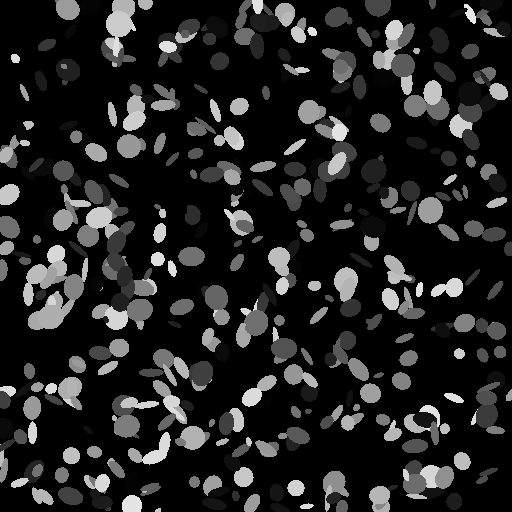
\includegraphics[width=60mm]{images/I-1.png}} ;
			\node<4> {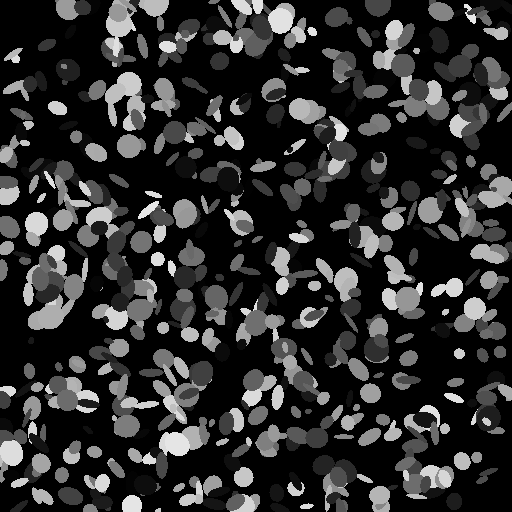
\includegraphics[width=60mm]{images/I-2.png}} ;
			\node<5> {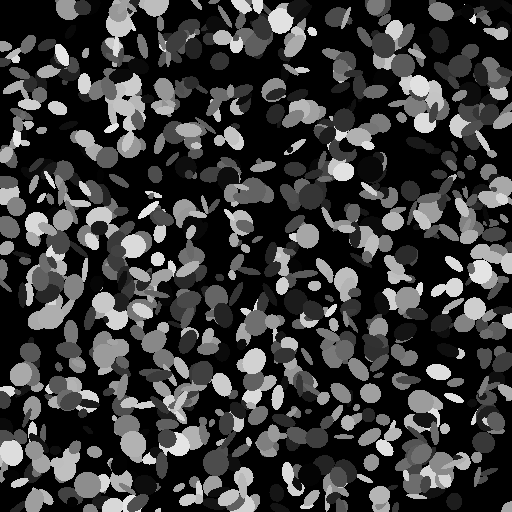
\includegraphics[width=60mm]{images/I-3.png}} ;
			\node<6> {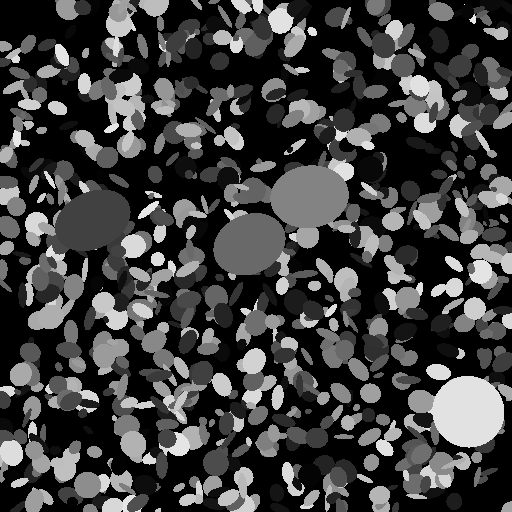
\includegraphics[width=60mm]{images/I-4.png}} ;
			\node<7> {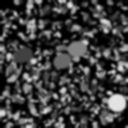
\includegraphics[width=60mm]{images/I-5.png}} ;
			% \node<8> {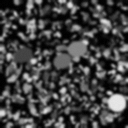
\includegraphics[width=60mm]{images/I-6.png}} ;
		\end{scope}
	\end{tikzpicture}
	\vfill
\end{frame}

\begin{frame}[t, label=GenSpecklesTransfo]
	\vspace{0mm}
	\centering
	\vfill
	\begin{tikzpicture}
		\linespread{1}% <--- locally defined vertical line spacing in nodes
		\drawBorder
		\nodePageNumber

		\onlystyle<2->{shd1}{myShaded}
		\onlystyle<4->{shd2}{myShaded}
		\onlystyle<5->{shd3}{myShaded}
		% \onlystyle<5->{shd4}{myShaded}
		% \onlystyle<6->{shd5}{myShaded}
		% \onlystyle<7->{shd6}{myShaded}
		\node<1-2>[shd1] at (\midX,85mm) {Trasnformations d'images} ;

		\begin{scope}[xshift=\midX, yshift=\midY+25mm]
			\node<2-> at (-31.5mm,0) {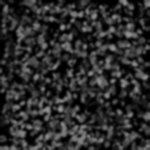
\includegraphics[width=15mm]{images/speckle_rot0.png}} ;
			\node<3-> at (-10.5mm,0) {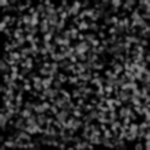
\includegraphics[width=15mm]{images/speckle_rot1.png}} ;
			\node<3-> at (10.5mm,0) {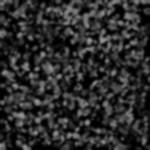
\includegraphics[width=15mm]{images/speckle_rot2.png}} ;
			\node<3-> at (31.5mm,0) {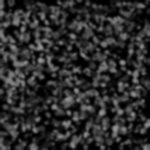
\includegraphics[width=15mm]{images/speckle_rot3.png}} ;
			\begin{scope}[xshift=0mm, yshift=8mm]
				\draw<3->[myarrow, shd2] (-31.5mm, 0) to[bend left] ++ (20mm, 0) ;
				\draw<3->[myarrow, shd2] (-10.5mm, 0) to[bend left] ++ (20mm, 0) ;
				\draw<3->[myarrow, shd2] (10.5mm, 0) to[bend left] ++ (20mm, 0) ;
				\node<3->[shd2] at (-21.5mm, 5mm) {rot 90°} ;
				\node<3->[shd2] at (-0.5mm, 5mm) {rot 90°} ;
				\node<3->[shd2] at (20.5mm, 5mm) {rot 90°} ;
			\end{scope}
			\draw<5-> [decorate, thick,decoration={brace,amplitude=5pt},xshift=0pt,yshift=0pt]
			(39.5mm,7mm) -- ++(0,-32mm) ;
			\draw<5-> [decorate, thick,decoration={brace,amplitude=5pt},xshift=0pt,yshift=0pt]
			(39.5mm,-29mm) -- ++(0,-32mm) ;
			\draw<5->[myarrow] (41.8mm, -9mm) to[bend left=10] ++ (0, -36mm) ;
			\node<5->[rotate=-90, text centered] at (47mm, -25mm) {1. - image} ;
		\end{scope}

		\begin{scope}[xshift=\midX, yshift=\midY+7mm]
			\node<4-> at (-31.5mm,0) {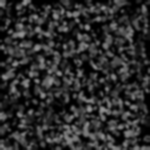
\includegraphics[width=15mm]{images/speckle_mirror_rot0.png}} ;
			\node<4-> at (-10.5mm,0) {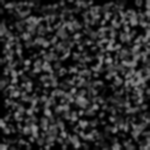
\includegraphics[width=15mm]{images/speckle_mirror_rot1.png}} ;
			\node<4-> at (10.5mm,0) {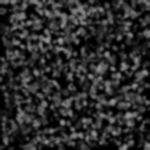
\includegraphics[width=15mm]{images/speckle_mirror_rot2.png}} ;
			\node<4-> at (31.5mm,0) {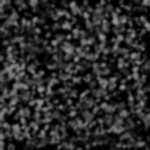
\includegraphics[width=15mm]{images/speckle_mirror_rot3.png}} ;
			\draw<4->[myarrow, shd3] (-39.5mm, 18mm) to[bend right] ++ (0, -20mm) ;
			\node<4->[shd3, rotate=90] at (-47mm, 7mm) {miroir horizontal} ;
		\end{scope}

		\begin{scope}[xshift=\midX, yshift=\midY-11mm]
			\node<5-> at (-31.5mm,0) {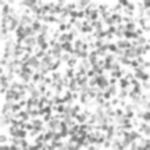
\includegraphics[width=15mm]{images/speckle_inv_rot0.png}} ;
			\node<5-> at (-10.5mm,0) {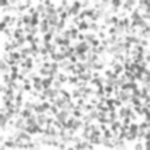
\includegraphics[width=15mm]{images/speckle_inv_rot1.png}} ;
			\node<5-> at (10.5mm,0) {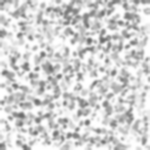
\includegraphics[width=15mm]{images/speckle_inv_rot2.png}} ;
			\node<5-> at (31.5mm,0) {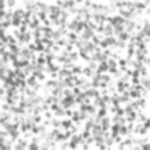
\includegraphics[width=15mm]{images/speckle_inv_rot3.png}} ;
		\end{scope}

		\begin{scope}[xshift=\midX, yshift=\midY-29mm]
			\node<5-> at (-31.5mm,0) {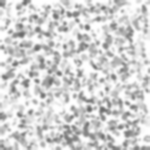
\includegraphics[width=15mm]{images/speckle_mirror_inv_rot0.png}} ;
			\node<5-> at (-10.5mm,0) {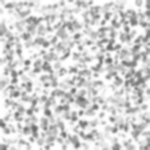
\includegraphics[width=15mm]{images/speckle_mirror_inv_rot1.png}} ;
			\node<5-> at (10.5mm,0) {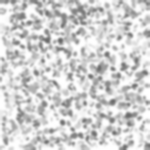
\includegraphics[width=15mm]{images/speckle_mirror_inv_rot2.png}} ;
			\node<5-> at (31.5mm,0) {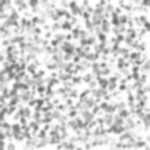
\includegraphics[width=15mm]{images/speckle_mirror_inv_rot3.png}} ;
		\end{scope}

		\node<6> at (\midX, 5mm) {\alert{1} image $\rightarrow$ \alert{16} images} ;
	\end{tikzpicture}
	\vfill
\end{frame}


\begin{frame}[t, label=GenImagesRefDef]
	\vspace{0mm}
	\centering
	\vfill
	\begin{tikzpicture}
		\linespread{1}% <--- locally defined vertical line spacing in nodes
		\drawBorder
		\nodePageNumber

		\onlystyle<2->{shd1}{myShaded}
		% \onlystyle<3->{shd2}{myShaded}
		% \onlystyle<4->{shd3}{myShaded}
		% \onlystyle<5->{shd4}{myShaded}
		% \onlystyle<6->{shd5}{myShaded}
		% \onlystyle<7->{shd6}{myShaded}
		\node[shd1] at (\midX,85mm) {Génération de pair d'images} ;

		\begin{scope}[xshift=\midX, yshift=\midY-5mm]
			\begin{scope}[yshift=25mm]
				\node<2-4> at (-22.5mm, 0) {Maillage dans repère de \alert{référence}} ;
				\node<2-4> at (22mm, 0){Image initiale} ;
				\node<5-> at (-15mm, 14mm) {Image de référence} ;
				\node<5-> at (15mm, 14mm) {Image déformée} ;
			\end{scope}
			
			\begin{scope}[yshift=-25mm]
				\node<3> {Interpolation de l'image de \alert{référence}} ;
				\node<4> {Interpolation de l'image \alert{déformée} sur un \textcolor{green}{maillage linéaire}} ;
			\end{scope}
			
			\node<2> {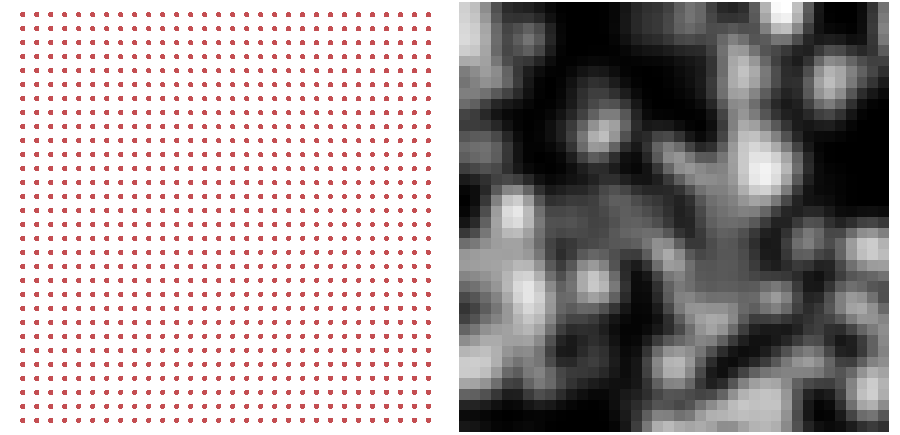
\includegraphics[width=90mm]{images/ref-0.pdf}} ;
			\node<3> {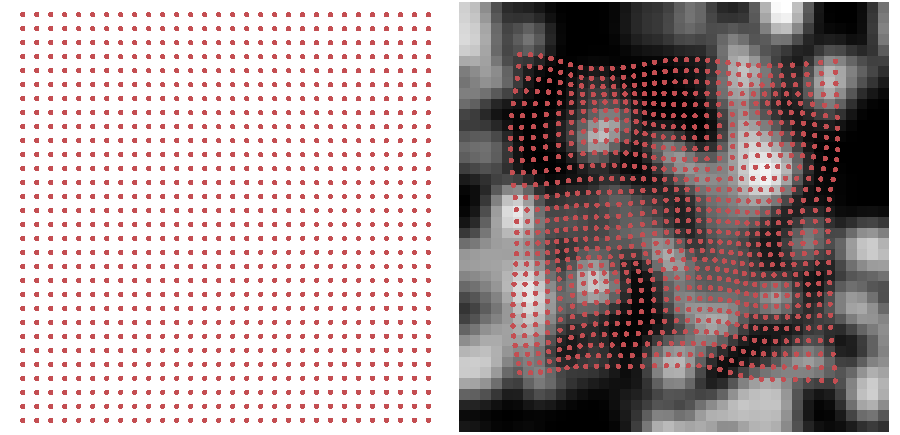
\includegraphics[width=90mm]{images/ref-1.pdf}} ;
			\node<4> {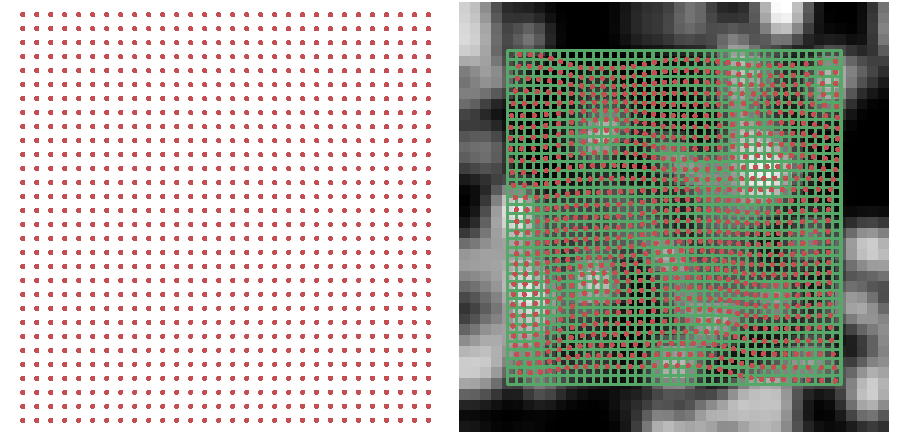
\includegraphics[width=90mm]{images/ref-def.pdf}} ;
			\node<5-> at (0, 21mm) {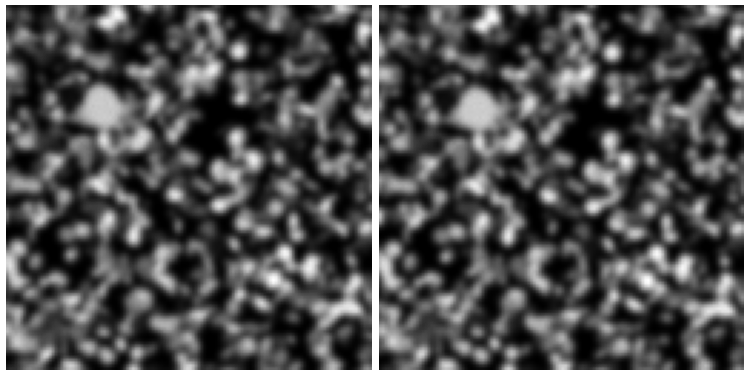
\includegraphics[width=60mm]{image_pair.pdf}} ;
			\node<6> at (0, -18mm) {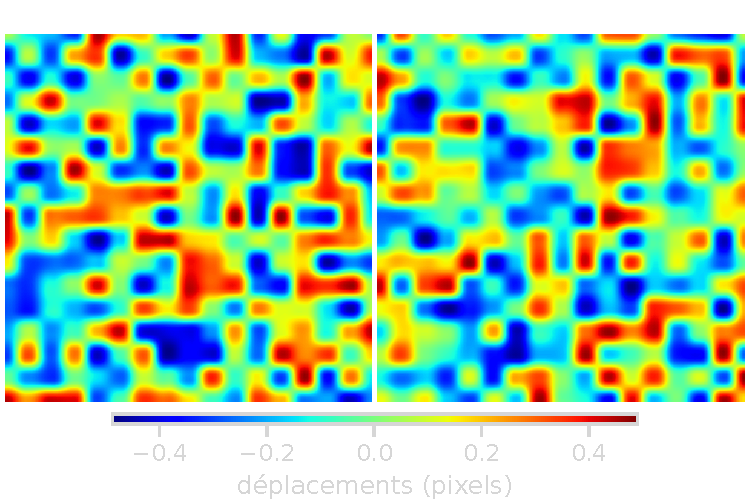
\includegraphics[width=60mm]{image_pair_deplacements.pdf}} ;
			\node<6-> at (-15mm, 2mm) {$\Delta u$} ;
			\node<6-> at (15mm, 2mm) {$\Delta v$} ;
		\end{scope}
	\end{tikzpicture}
	\vfill
\end{frame}


\section{MODÉLISATION}
\subsection{Modèle initiale}
\begin{frame}[t, label=ArchitectureGenerale]
	\vspace{0mm}
	\centering
	\vfill
	\begin{tikzpicture}
		\linespread{1}% <--- locally defined vertical line spacing in nodes
		\drawBorder
		\nodePageNumber

		\onlystyle<2->{shd1}{myShaded}
		% \onlystyle<3->{shd2}{myShaded}
		% \onlystyle<4->{shd3}{myShaded}
		% \onlystyle<5->{shd4}{myShaded}
		% \onlystyle<6->{shd5}{myShaded}
		% \onlystyle<7->{shd6}{myShaded}
		\node<1>[shd1] at (\midX,80mm) {Architecture} ;

		\begin{scope}[xshift=\midX-14.5mm, yshift=\midY+38mm, every node/.append style={transform shape}, scale=0.7]
			\tikzset{concatenation/.style={box, fill=cyan!60, text=black}}
			\tikzset{dconv/.style={box, fill=green!60, text=black}}
			\tikzset{residuel/.style={box, fill=red!80}}

			\visible<2->{
				\node[box,minimum height=6mm] (X) {Paire d'image};
			}
    
			\visible<17->{
				\node[box, right= of X, xshift=5mm, minimum height=6mm,] (Y) {Déplacement / Déformation} ;
			}
			\visible<16->{
				\node[box, below= of Y, yshift=5mm] (convLast) {Separable Conv2d} ;
			}
			\draw<17->[myarrow] (convLast) -- (Y) ;
			
			% CONCAT 0
			\visible<15->{
				\node[concatenation, below= of convLast, yshift=5mm] (concat0) {Concaténation} ;
			}
			\draw<16->[myarrow] (concat0) -- (convLast) ;

			\visible<3->{
				\node[box, below=of X,, yshift=5mm] (RPE) {Extracteur de Position Relative} ;
			}
			\draw<3->[myarrow] (X) -- (RPE) ;
			\draw<15->[myarrow] (RPE) |- (concat0) ;

			% DOUBLE CONV 0
			\visible<15->{
				\node[dconv, below= of concat0, yshift=7mm] (dblConv0) {Upsample - Double Conv2d} ;
			}
			\draw<15->[myarrow] (dblConv0) -- (concat0) ;

			% CONCAT 1
			\visible<14->{
				\node[concatenation, below= of dblConv0, yshift=-1mm] (concat1) {Concaténation} ;
			}
			\draw<15->[myarrow] (concat1) -- (dblConv0) ;

			% DOUBLE CONV 1
			\visible<14->{
				\node[dconv, below= of concat1, yshift=7mm] (dblConv1) {Upsample - Double Conv2d} ;
			}
			\draw<14->[myarrow] (dblConv1) -- (concat1) ;

			% CONCAT 2
			\visible<13->{
				\node[concatenation, below= of dblConv1, yshift=4mm] (concat2) {Concaténation} ;
			}
			\draw<14->[myarrow] (concat2) -- (dblConv1) ;


			% DOUBLE CONV 2
			\visible<13->{
				\node[dconv, below= of concat2, yshift=7mm] (dblConv2) {Upsample - Double Conv2d} ;
			}
			\draw<13->[myarrow] (dblConv2) -- (concat2) ;

			% CONCAT 3
			\visible<12->{
				\node[concatenation, below= of dblConv2, yshift=4mm] (concat3) {Concaténation} ;
			}
			\draw<13->[myarrow] (concat3) -- (dblConv2) ;

			% DOUBLE CONV 3
			\visible<12->{
				\node[dconv, below= of concat3, yshift=7mm] (dblConv3) {Upsample - Double Conv2d} ;
			}
			\draw<12->[myarrow] (dblConv3) -- (concat3) ;

			% CONCAT 4
			\visible<11->{
				\node[concatenation, below= of dblConv3, yshift=4mm] (concat4) {Concaténation} ;
			}
			\draw<12->[myarrow] (concat4) -- (dblConv3) ;

			% DOUBLE CONV 4
			\visible<10->{
				\node[dconv, below= of concat4, yshift=7mm] (dblConv4) {Upsample - Double Conv2d} ;
			}
			\draw<11->[myarrow] (dblConv4) -- (concat4) ;

			% RES 1
			\visible<4->{
				\node[residuel, below=of RPE, yshift=-2mm] (Res1) {Module résiduel (s:2)} ;
			}
			\draw<4->[myarrow] (RPE) -- (Res1) ;
			\node<4->[right=of Res1, xshift=-10mm] {$\times$~1} ;

			% RES 2
			\visible<5->{
				\node[residuel, below=of Res1, yshift=6mm] (Res2) {Module résiduel (s:1)} ;
			}
			\draw<5->[myarrow] (Res1) -- (Res2) ;
			\draw<14->[myarrow] (Res2) |- (concat1) ;
			\node<5->[right=of Res2, xshift=-10mm] {$\times$~5} ;

			% RES 3
			\visible<6->{
				\node[residuel, below=of Res2, yshift=-2mm] (Res3) {Module résiduel (s:2)} ;
			}
			\draw<6->[myarrow] (Res2) -- (Res3) ;
			\draw<13->[myarrow] (Res3) |- (concat2) ;
			\node<6->[right=of Res3, xshift=-10mm] {$\times$~6} ;
			
			% RES 4
			\visible<7->{
				\node[residuel, below=of Res3, yshift=-2mm] (Res4) {Module résiduel (s:2)} ;
			}
			\draw<7->[myarrow] (Res3) -- (Res4) ;
			\draw<12->[myarrow] (Res4) |- (concat3) ;
			\node<7->[right=of Res4, xshift=-10mm] {$\times$~8} ;
			
			% RES 5
			\visible<8->{
				\node[residuel, below=of Res4, yshift=-3mm] (Res5) {Module résiduel (s:2)} ;
			}
			\draw<8->[myarrow] (Res4) -- (Res5) ;
			\draw<11->[myarrow] (Res5) |- (concat4) ;
			\node<8->[right=of Res5, xshift=-10mm] {$\times$~5} ;
			
			% RES 6
			\visible<9->{
				\node[residuel, below=of Res5, yshift=-2mm] (Res6) {Module résiduel (s:2)} ;
			}
			\draw<9->[myarrow] (Res5) -- (Res6) ;
			\draw<10->[myarrow] (Res6) -- ++ (0, -8mm) -| (dblConv4) ;
			\node<9->[right=of Res6, xshift=-10mm] {$\times$~3} ;
		\end{scope}

	\end{tikzpicture}
	\vfill
\end{frame}


\begin{frame}[t, label=ResidualDoubleConv]
	\vspace{0mm}
	\centering
	\vfill
	\begin{tikzpicture}
		\linespread{1}% <--- locally defined vertical line spacing in nodes
		\drawBorder
		\nodePageNumber

		\onlystyle<2->{shd1}{myShaded}
		\onlystyle<11->{shd2}{myShaded}
		% \onlystyle<4->{shd3}{myShaded}
		% \onlystyle<5->{shd4}{myShaded}
		% \onlystyle<6->{shd5}{myShaded}
		% \onlystyle<7->{shd6}{myShaded}
		\begin{scope}[xshift=\midX-22mm]
			\node[shd1] at (0,85mm) {Module résiduel:} ;
			\begin{scope}[xshift=0mm, yshift=\midY+30mm, every node/.append style={transform shape}, scale=0.9]
				\tikzset{conv/.style={box, fill=red!80, text width=31mm}}
				\tikzset{norm/.style={box, fill=yellow!100, text=black, text width=31mm}}

				\node<2->[box] (X) {Entrée};
    
				\node<3->[conv, below=of X] (conv1) {Conv2d (1~$\times$~1)} ;
				\draw<3->[myarrow] (X) -- (conv1) ;
				
				\node<4->[norm, below=of conv1, yshift=5mm] (norm1) {Batch Norm et ReLU} ;
				\draw<4->[myarrow] (conv1) -- (norm1) ;

				\node<5->[conv, below=of norm1, yshift=5mm] (conv2) {Conv2d (3~$\times$~3), stride} ;
				\draw<5->[myarrow] (norm1) -- (conv2) ;

				\node<6->[norm, below=of conv2, yshift=5mm] (norm2) {Batch Norm et ReLU} ;
				\draw<6->[myarrow] (conv2) -- (norm2) ;

				\node<7->[conv, below=of norm2, yshift=5mm] (conv3) {Conv2d (1~$\times$~1)} ;
				\draw<7->[myarrow] (norm2) -- (conv3) ;
				
				\node<8->[draw, circle, minimum height= 5mm, below=of conv3, yshift=5mm] (add) {+} ;
				\draw<8->[myarrow] (conv3) -- (add) ;
				\draw<8->[myarrow] (X) -- ++ (0, -7mm) -| ++ (-22mm, -15mm) |- (add) ;
				\node<9->[box, below=of add, yshift=5mm] (Y) {Sortie} ;
				\draw<9->[myarrow] (add) -- (Y) ;
			\end{scope}
		\end{scope}

		\begin{scope}[xshift=\midX+22mm]
			\node<10->[shd2] at (0,85mm) {Module double conv:} ;
			\begin{scope}[xshift=0mm, yshift=\midY-30mm, every node/.append style={transform shape}, scale=0.9]
				\tikzset{conv/.style={box, fill=red!80, text width=30mm}}
				\tikzset{norm/.style={box, fill=yellow!100, text=black, text width=30mm}}
				\tikzset{upsample/.style={box, fill=green!60, text=black, text width=30mm}}

				\node<11->[box] (X) {Entrée};
    
				\node<12->[upsample, above=of X] (up1) {Sur-échantillonnage} ;
				\draw<12->[myarrow] (X) -- (up1) ;
				
				\node<13->[conv, above=of up1, yshift=-5mm] (conv1) {Conv2d (3~$\times$~3)} ;
				\draw<13->[myarrow] (up1) -- (conv1) ;
				
				\node<14->[norm, above=of conv1, yshift=-5mm] (norm1) {ReLU} ;
				\draw<14->[myarrow] (conv1) -- (norm1) ;

				\node<15->[conv, above=of norm1, yshift=-5mm] (conv2) {Conv2d (3~$\times$~3)} ;
				\draw<15->[myarrow] (norm1) -- (conv2) ;
				
				\node<16->[norm, above=of conv2, yshift=-5mm] (norm2) {ReLU} ;
				\draw<16->[myarrow] (conv2) -- (norm2) ;
				
				\node<17->[box, above=of norm2] (Y) {Sortie};
				\draw<17->[myarrow] (norm2) -- (Y) ;
			\end{scope}
		\end{scope}

	\end{tikzpicture}
	\vfill
\end{frame}

\begin{frame}[t, label=HyperParameters]
	\vspace{0mm}
	\centering
	\vfill
	\begin{tikzpicture}
		\linespread{1}% <--- locally defined vertical line spacing in nodes
		\drawBorder
		\nodePageNumber

		\onlystyle<2->{shd1}{myShaded}
		\onlystyle<3->{shd2}{myShaded}
		\onlystyle<4->{shd3}{myShaded}
		\onlystyle<5->{shd4}{myShaded}
		% \onlystyle<6->{shd5}{myShaded}
		% \onlystyle<7->{shd6}{myShaded}
		\node[shd1] at (\midX,80mm) {Paramètres d'entrainement~:} ;

		\node<2->[shd2] at (\midX,\midY+25mm) {Optimiseur~: Adam, $\beta_1$=0,9, $\beta_2$=0.999, $\lambda$=0} ;
		\node<3->[shd3] at (\midX,\midY+15mm) {Jeu d'entrainement~: $N_0$=200 $\rightarrow$ 3200 paires d'images} ;
		\node<4->[shd4] at (\midX,\midY+5mm) {Jeu de test~: $N_0$=20 $\rightarrow$ 320 paires d'images} ;
		\node<5-> at (\midX,\midY-5mm) {$lr = 10^{-5} * (1 + 9 * 0,94^{\text{\textit{étape}}})$} ;
		\node<5-> at (\midX,\midY-25mm) {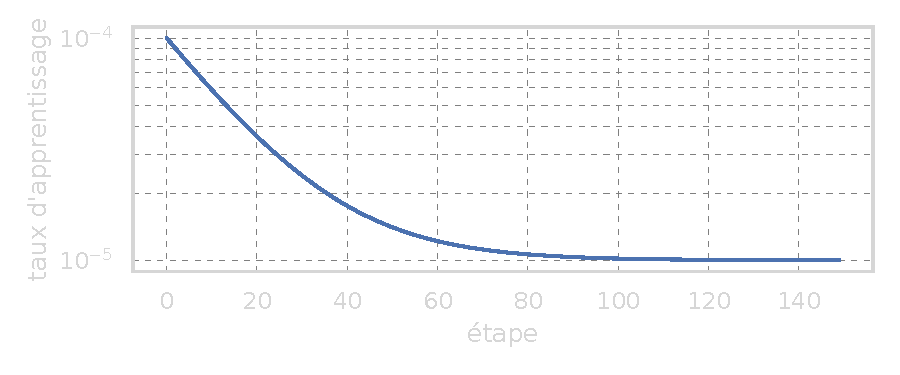
\includegraphics[width=80mm]{lr.pdf}} ;
	\end{tikzpicture}
	\vfill
\end{frame}

\begin{frame}[t, label=Results1]
	\vspace{0mm}
	\centering
	\vfill
	\begin{tikzpicture}
		\linespread{1}% <--- locally defined vertical line spacing in nodes
		\drawBorder
		\nodePageNumber

		\onlystyle<2->{shd1}{myShaded}
		% \onlystyle<3->{shd2}{myShaded}
		% \onlystyle<4->{shd3}{myShaded}
		% \onlystyle<5->{shd4}{myShaded}
		% \onlystyle<6->{shd5}{myShaded}
		% \onlystyle<7->{shd6}{myShaded}
		\node[shd1] at (\midX,85mm) {Résultats d'entrainement~:} ;

		\begin{scope}[xshift=\midX, yshift=72mm]
			\node<3->[box, myOrng, text width=25mm] at (-35mm,0) {Batch Norm\\$\downarrow$\\Group Norm (4)} ;
			\node<5->[box, green!60, text width=25mm] at (0mm,0) {Batch 16\\$\downarrow$\\Batch 1} ;
			\node<7->[box, red!60, text width=25mm] at (35mm,0) {ReLU\\$\downarrow$\\Mish} ;
		\end{scope}

		\begin{scope}[xshift=\midX, yshift=\midY-10mm]
			\node {
				\includegraphics<2-3>[width=80mm]{results-1/training_1.pdf}%
				\includegraphics<4-5>[width=80mm]{results-1/training_2.pdf}%
				\includegraphics<6-7>[width=80mm]{results-1/training_3.pdf}%
				\includegraphics<8>[width=80mm]{results-1/training_4.pdf}%
			} ;
		\end{scope}
	\end{tikzpicture}
	\vfill
\end{frame}

\subsection{Modifications du réseau}
\begin{frame}[t, label=modifs2]
	\vspace{0mm}
	\centering
	\vfill
	\begin{tikzpicture}
		\linespread{1}% <--- locally defined vertical line spacing in nodes
		\drawBorder
		\nodePageNumber

		\onlystyle<2->{shd1}{myShaded}
		\onlystyle<3->{shd2}{myShaded}
		\onlystyle<4->{shd3}{myShaded}
		% \onlystyle<5->{shd4}{myShaded}
		% \onlystyle<6->{shd5}{myShaded}
		% \onlystyle<7->{shd6}{myShaded}
		\node[shd1] at (\midX,85mm) {Modifications de la structure~: module de convolution dense} ;

		\begin{scope}[xshift=\midX, yshift=\midY, every node/.append style={transform shape}]
			\visible<2->{
			\begin{scope}[xshift=-32.5mm, yshift=25mm, scale=0.8, node distance=7mm]
				\tikzset{conv/.style={box, fill=red!80, text width=25mm}}
				\tikzset{norm/.style={box, fill=yellow!100, text=black, text width=25mm}}
				\tikzset{concatenation/.style={box, fill=cyan!60, text width=25mm}}
				
				\node[shd2, text width=30mm, text centered] at (0, 10mm) {Bloc\\example 3 couches} ;
				\node[box] (X) {Entrée ($N_0$)};
		
				\node[conv, below=of X] (conv1) {Dense Conv2d layer ($N_1:N_0+k$)} ;
				\draw[myarrow] (X) -- (conv1) ;
				
				\node[conv, below=of conv1] (conv2) {Dense Conv2d layer ($N_2: N_1+k$)} ;
				\draw[myarrow] (conv1) -- (conv2) ;
	
				\node[conv, below=of conv2] (conv3) {Dense Conv2d layer ($N_3: N_2+k$)} ;
				\draw[myarrow] (conv2) -- (conv3) ;
				
				\node[norm, below=of conv3] (transition) {Transition layer ($N: N_3 // 2$)} ;
				\draw[myarrow] (conv3) -- (transition) ;
				
				% \draw[myarrow] (conv3) -- (add) ;
				% \draw[myarrow] (X) -- ++ (0, -7mm) -| ++ (-25mm, -15mm) |- (add) ;
				
				\node[box, below=of transition] (Y) {Sortie} ;
				\draw[myarrow] (transition) -- (Y) ;
			\end{scope}
			}

			\visible<3->{
			\begin{scope}[xshift=0mm, yshift=25mm, scale=0.8, node distance=7mm]
				\tikzset{conv/.style={box, fill=red!80, text width=25mm}}
				\tikzset{norm/.style={box, fill=yellow!100, text=black, text width=25mm}}
				\tikzset{concatenation/.style={box, fill=cyan!60, text width=25mm}}
				
				\node[shd3, text centered, text width=30mm] at (0, 10mm) {Couche\\Dense Conv2d} ;
				\node[box] (X) {Entrée};
    
				\node[conv, below=of X, yshift=-3mm] (conv1) {Conv2d (1$\times$1), N:$16k$} ;
				\draw[myarrow] (X) -- (conv1) ;
				
				\node[conv, below=of conv1] (conv2) {Conv2d (3$\times$3), N:$k$, s:1, pad:1} ;
				\draw[myarrow] (conv1) -- (conv2) ;
			
			
				\node[norm, below=of conv2] (norm3) {Group Norm (4), Mish activation} ;
				\draw[myarrow] (conv2) -- (norm3) ;
				
				\node[box, below=of norm3, yshift=-3mm] (Y) {Sortie} ;
				\draw[myarrow] (norm3) -- (Y) ;
			
				\draw[myarrow] (X)  |- ++ (-20mm, -7mm) -- ++ (0, -47mm) -| (Y) ;
			\end{scope}
			}

			\visible<4->{
			\begin{scope}[xshift=32.5mm, yshift=25mm, scale=0.8, node distance=7mm]
				\tikzset{conv/.style={box, fill=red!80, text width=25mm}}
				\tikzset{norm/.style={box, fill=yellow!100, text=black, text width=25mm}}
				\tikzset{concatenation/.style={box, fill=cyan!60, text width=25mm}}
				
				\node[shd3, text centered, text width=30mm] at (0, 10mm) {Cocuhe de \\Transition} ;
				\node[box] (X) {Entrée, $N_0$};
    
				\node[conv, below=of X] (conv1) {Conv2d (1$\times$1), N:$N_0//2$} ;
				\draw[myarrow] (X) -- (conv1) ;
				
				\node[norm, below=of conv1] (norm2) {Group Norm (4), Mish activation} ;
				\draw[myarrow] (conv1) -- (norm2) ;

				\node[conv, below=of norm2] (AvgPool) {Average pooling (s$\times$s), stride:s} ;
				\draw[myarrow] (norm2) -- (AvgPool) ;
				
				\node[box, below=of AvgPool] (Y) {Sortie} ;
				\draw[myarrow] (AvgPool) -- (Y) ;
			\end{scope}
			}
		\end{scope}

	\end{tikzpicture}
	\vfill
\end{frame}

\begin{frame}[t, label=modifs22]
	\vspace{0mm}
	\centering
	\vfill
	\begin{tikzpicture}
		\linespread{1}% <--- locally defined vertical line spacing in nodes
		\drawBorder
		\nodePageNumber

		\onlystyle<2->{shd1}{myShaded}
		% \onlystyle<3->{shd2}{myShaded}
		% \onlystyle<4->{shd3}{myShaded}
		% \onlystyle<5->{shd4}{myShaded}
		% \onlystyle<6->{shd5}{myShaded}
		% \onlystyle<7->{shd6}{myShaded}
		\node[shd1, text centered, text width=50mm] at (\midX,80mm) {Modifications du réseau~:\\convolution séparable augmentée} ;

		\visible<2->{
		\begin{scope}[xshift=\midX-20mm, yshift=\midY+20mm, every node/.append style={transform shape}, scale=0.8, node distance=7mm]
			\tikzset{conv/.style={box, fill=red!80, text width=30mm}}
			\tikzset{norm/.style={box, fill=yellow!100, text=black, text width=30mm}}
			\tikzset{concatenation/.style={box, fill=cyan!60, text width=30mm}}

			\node[box] (X) {Entrée, $N_0$};
    
			\node[conv, below=of X] (conv1) {Conv2d (3$\times$3),\\N:$n*N_0$, g:$N_0$, s:1, pad:1} ;
			\draw[myarrow] (X) -- (conv1) ;
			
			\node[conv, below=of conv1] (conv2) {Conv2d (1$\times$1), N:$N_{out}$} ;
			\draw[myarrow] (conv1) -- (conv2) ;


			\node[norm, below=of conv2] (norm3) {Group Norm (4), Mish activation} ;
			\draw[myarrow] (conv2) -- (norm3) ;
			
			\node[box, below=of norm3] (Y) {Sortie} ;
			\draw[myarrow] (norm3) -- (Y) ;
		\end{scope}
		}
		\begin{scope}[xshift=\midX+20mm, yshift=\midY]
			\node<3>[box, text width=40mm] at (0,0mm) {Remplacement dans les couches de \alert{convolutions dense} et de \alert{double convolutions}} ;
		\end{scope}

	\end{tikzpicture}
	\vfill
\end{frame}

\begin{frame}[t, label=modifs23]
	\vspace{0mm}
	\centering
	\vfill
	\begin{tikzpicture}
		\linespread{1}% <--- locally defined vertical line spacing in nodes
		\drawBorder
		\nodePageNumber

		\onlystyle<2->{shd1}{myShaded}
		\onlystyle<11->{shd2}{myShaded, text=myShaded}
		\definecolor{redshaded}{rgb}{0.6,0,0}
		\onlystyle<11->{shd2Text}{text=myShaded, fill=redshaded}
		\onlystyle<12->{shd3}{myShaded}
		% \onlystyle<5->{shd4}{myShaded}
		% \onlystyle<6->{shd5}{myShaded}
		% \onlystyle<7->{shd6}{myShaded}
		\node[shd1, text centered, text width=50mm] at (\midX,80mm) {Modifications du réseau~:\\convolution partagée intriquée} ;

		\begin{scope}[shd2, xshift=\midX-20mm, yshift=\midY+25mm, every node/.append style={transform shape}, scale=0.8, node distance=7mm]
			\tikzset{conv/.style={box, fill=red!80, text width=30mm, shd2Text}}
			\tikzset{box2/.style={box, text width=30mm, shd2}}

			\node<2->[box2] (X) {Entrée\\$N \times C \times H \times W$};

			\node<3->[box2, below=of X, yshift=-5mm, xshift=-20mm] (X2) {Redimensionnement $N*C \times 1 \times H \times W$} ;
			\draw<3->[myarrow] (X.south) -- ++ (0mm, -6mm) -| (X2) ;
			

			\node<4->[conv, below=of X2] (conv1) {Conv2d (3$\times$3), N:$N_f$\\$N*C \times N_f \times H \times W$} ;
			\draw<4->[myarrow] (X2) -- (conv1) ;
			

			\node<5->[box2, below=of conv1] (swap1) {Échange d'axes\\$N_f \times N*C \times H \times W$} ;
			\draw<5->[myarrow] (conv1) -- (swap1) ;

			\node<6->[box2, below=of swap1] (reshape1) {Redimensionnement\\$N_f \times N \times C \times H \times W$} ;
			\draw<6->[myarrow] (swap1) -- (reshape1) ;

			\node<7->[box2, below=of X, xshift=25mm] (swap2) {Échange d'axes\\$N \times N_f \times C \times H \times W$} ;
			\draw<7->[myarrow] (reshape1.south) |- ++ (25mm, -5mm) -- ++(0, 68mm) -| (swap2) ;

			\node<8->[box2, below=of swap2] (reshape2) {Redimensionnement\\$N \times N_f * C \times H \times W$} ;
			\draw<8->[myarrow, shd2] (swap2) -- (reshape2) ;
			
			\node<9->[conv, below=of reshape2] (conv2) {Conv2d (1$\times$1) N:$N_f$, g:$N_f$\\$N \times N_f \times H \times W$} ;
			\draw<9->[myarrow] (reshape2) -- (conv2) ;

			\node<10->[box2, below=of conv2] (Y) {Sortie\\$N \times N_f \times H \times W$} ;
			\draw<10->[myarrow] (conv2) -- (Y) ;
		\end{scope}

		\begin{scope}[xshift=\midX+33mm, yshift=\midY]
			\node<11->[box, shd3, text width=28.5mm] at (0,10mm) {Chaque \alert{groupe} de filtres (1~$\times$~1) est appliqué sur \alert{$C$ cartes}} ;
			\node<12->[box, text width=28.5mm] at (0,-10mm) {Appliqué uniquement en \alert{entrée} du \alert{réseau}} ;
		\end{scope}
	\end{tikzpicture}
	\vfill
\end{frame}

\begin{frame}[t, label=Results2]
	\vspace{0mm}
	\centering
	\vfill
	\begin{tikzpicture}
		\linespread{1}% <--- locally defined vertical line spacing in nodes
		\drawBorder
		\nodePageNumber

		\onlystyle<2->{shd1}{myShaded}
		\onlystyle<5->{shd2}{myShaded}
		% \onlystyle<4->{shd3}{myShaded}
		% \onlystyle<5->{shd4}{myShaded}
		% \onlystyle<6->{shd5}{myShaded}
		% \onlystyle<7->{shd6}{myShaded}
		\node[shd1] at (\midX,80mm) {Modifications du réseau} ;

		% \begin{scope}[xshift=\midX, yshift=72mm]
		% 	\node<2->[box, myOrng, text width=25mm] at (-35mm,0) {Batch Norm\\$\downarrow$\\Group Norm (4)} ;
		% 	\node<3->[box, green!60, text width=25mm] at (0mm,0) {Batch 16\\$\downarrow$\\Batch 1} ;
		% 	\node<4->[box, red!60, text width=25mm] at (35mm,0) {ReLU\\$\downarrow$\\Mish} ;
		% \end{scope}

		\begin{scope}[xshift=\midX, yshift=\midY-0mm]
			\node {
				% \includegraphics<5>[width=80mm]{results-2/training_1.pdf}%
				% \includegraphics<6>[width=80mm]{results-2/training_2.pdf}%
				\includegraphics<2>[width=80mm]{results-2/training_3.pdf}%
				\includegraphics<3>[width=80mm]{results-2/training_4.pdf}%
				\includegraphics<4->[width=80mm]{results-2/training_5.pdf}%
			} ;
			\node<6->[text centered, myOrng, font=\bfseries] (A) at (15mm,8mm) {Limitation mathématique ?} ;
			\draw<6->[myarrow, myOrng] (A) -- (10mm, -17mm) ;
			\draw<6->[dashed, thick, myOrng] (10mm, -14mm) -- ++ (25mm, -3mm) ;
			\draw<6->[myarrow, myOrng] (A) -- (28mm, -15.5mm) ;
		\end{scope}
		\node<5->[shd2] at (\midX,10mm) {\alert{Amélioration} significative des \alert{résultats}} ;
	\end{tikzpicture}
	\vfill
\end{frame}

\section{COMPARAISON DE DIFFÉRENTS MODÈLES}
\subsection{Images simulées}
\begin{frame}[t, label=Comparaison1]
	\vspace{0mm}
	\centering
	\vfill
	\begin{tikzpicture}
		\linespread{1}% <--- locally defined vertical line spacing in nodes
		\drawBorder
		\nodePageNumber

		\onlystyle<2->{shd1}{myShaded}
		\onlystyle<6->{shd2}{myShaded}
		% \onlystyle<4->{shd3}{myShaded}
		% \onlystyle<5->{shd4}{myShaded}
		% \onlystyle<6->{shd5}{myShaded}
		% \onlystyle<7->{shd6}{myShaded}
		\node[shd1] at (\midX,80mm) {Comparaison de modèles~:} ;

		\begin{scope}[xshift=\midX, yshift=\midY+17mm]
			\node<2->[box, shd2] (X) {Premier essais~: 1 pair d'images} ;
			\node<2->[left=of X.south, xshift=5mm, yshift=1.1mm] (XA) {} ;
			\node<2->[right=of X.south, xshift=-5mm, yshift=1.1mm] (XC) {} ;
		\end{scope}

		\begin{scope}[xshift=\midX, yshift=\midY-8mm]
			\node<3->[box, shd2] (A) at (-35mm,0) {Modèle proposé} ;
			\draw<3->[myarrow, shd2] (XA) -- ++ (0, -10mm) -| (A) ;
			\node<4->[box, shd2, text width=25mm] (B) at (0mm,0) {Corrélation d'image numériques\\(baseline)\\(21~$\times$~21 pixels)} ;
			\draw<4->[myarrow, shd2] (X) -- (B) ;
			\node<5->[box, shd2] (C) at (35mm,0) {Deep-DIC} ;
			\draw<5->[myarrow, shd2] (XC) -- ++ (0, -10mm) -| (C) ;
		\end{scope}

		\begin{scope}[xshift=\midX, yshift=\midY-30mm]
			\node<6->[box] (X) {Sorties~: \alert{cartes} de \alert{déplacements} et \alert{déformations}} ;
		\end{scope}
	\end{tikzpicture}
	\vfill
\end{frame}

\begin{frame}[t, label=ComparaisonStats]
	\vspace{0mm}
	\centering
	\vfill
	\begin{tikzpicture}
		\linespread{1}% <--- locally defined vertical line spacing in nodes
		\drawBorder
		\nodePageNumber

		\onlystyle<2->{shd1}{myShaded}
		% \onlystyle<3->{shd2}{myShaded}
		% \onlystyle<4->{shd3}{myShaded}
		% \onlystyle<5->{shd4}{myShaded}
		% \onlystyle<6->{shd5}{myShaded}
		% \onlystyle<7->{shd6}{myShaded}
		\node[shd1] at (\midX,80mm) {Comparaison de modèles~: statistiques} ;

		\begin{scope}[xshift=\midX, yshift=\midY-5mm]
			\node<2> {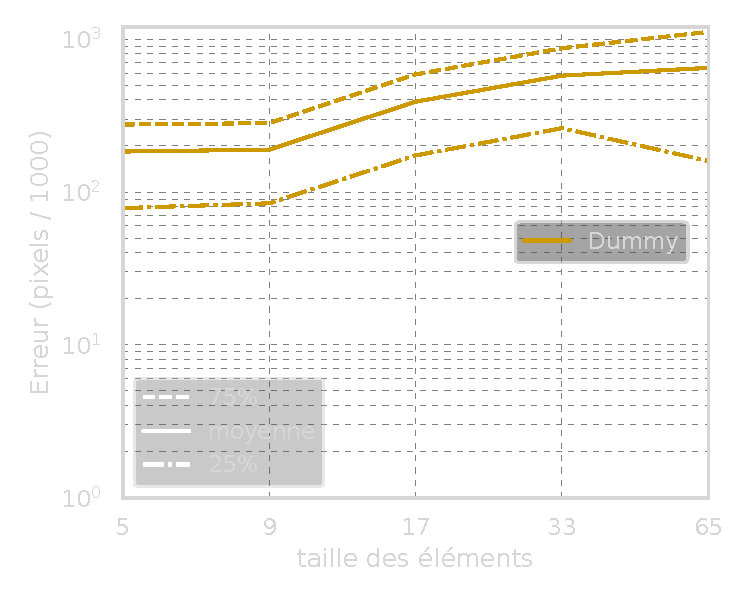
\includegraphics[width=80mm]{results_disp_0.pdf}} ;
			\node<3> {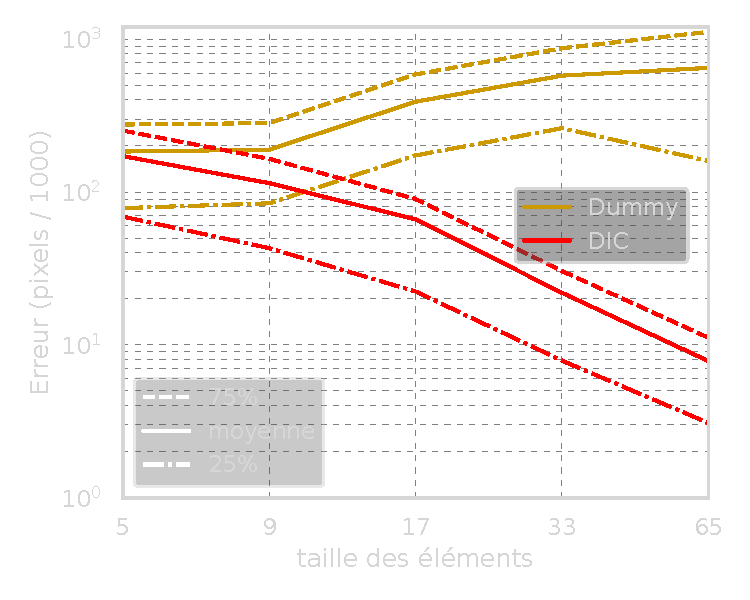
\includegraphics[width=80mm]{results_disp_1.pdf}} ;
			\node<4> {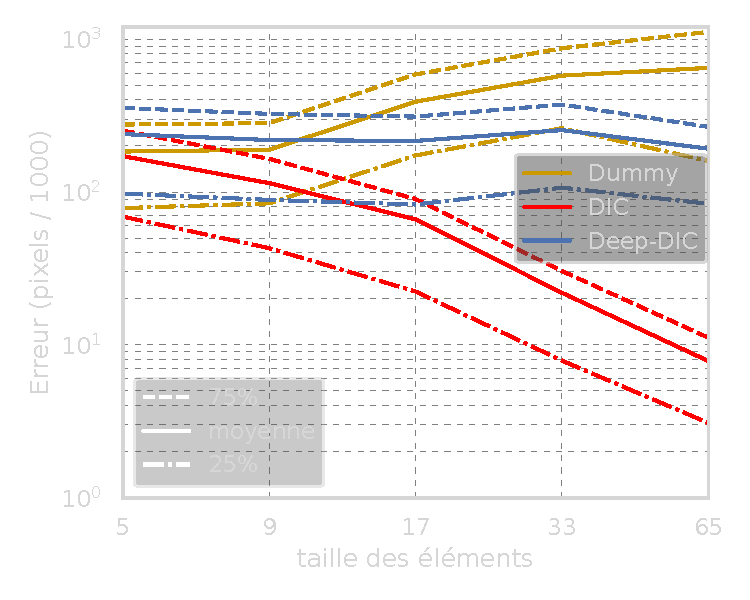
\includegraphics[width=80mm]{results_disp_2.pdf}} ;
			\node<5> {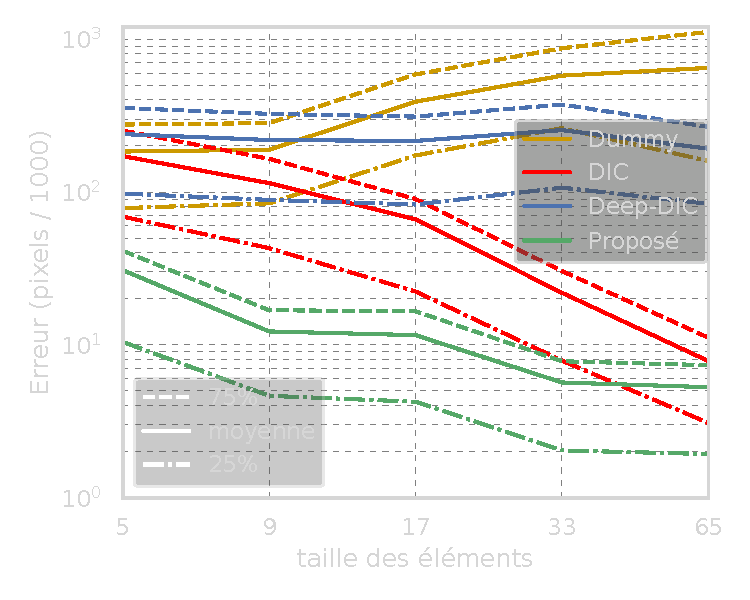
\includegraphics[width=80mm]{results_disp_3.pdf}} ;
		\end{scope}
	\end{tikzpicture}
	\vfill
\end{frame}


\begin{frame}[t, label=ComparaisonMaps]
	\vspace{0mm}
	\centering
	\vfill
	\begin{tikzpicture}
		\linespread{1}% <--- locally defined vertical line spacing in nodes
		\drawBorder
		\nodePageNumber

		\onlystyle<2->{shd1}{myShaded}
		% \onlystyle<3->{shd2}{myShaded}
		% \onlystyle<4->{shd3}{myShaded}
		% \onlystyle<5->{shd4}{myShaded}
		% \onlystyle<6->{shd5}{myShaded}
		% \onlystyle<7->{shd6}{myShaded}
		\node[shd1] at (\midX,85mm) {Comparaison de modèles~: cartes} ;

		\begin{scope}[xshift=\midX, yshift=\midY-5mm]
			\node<2-3> {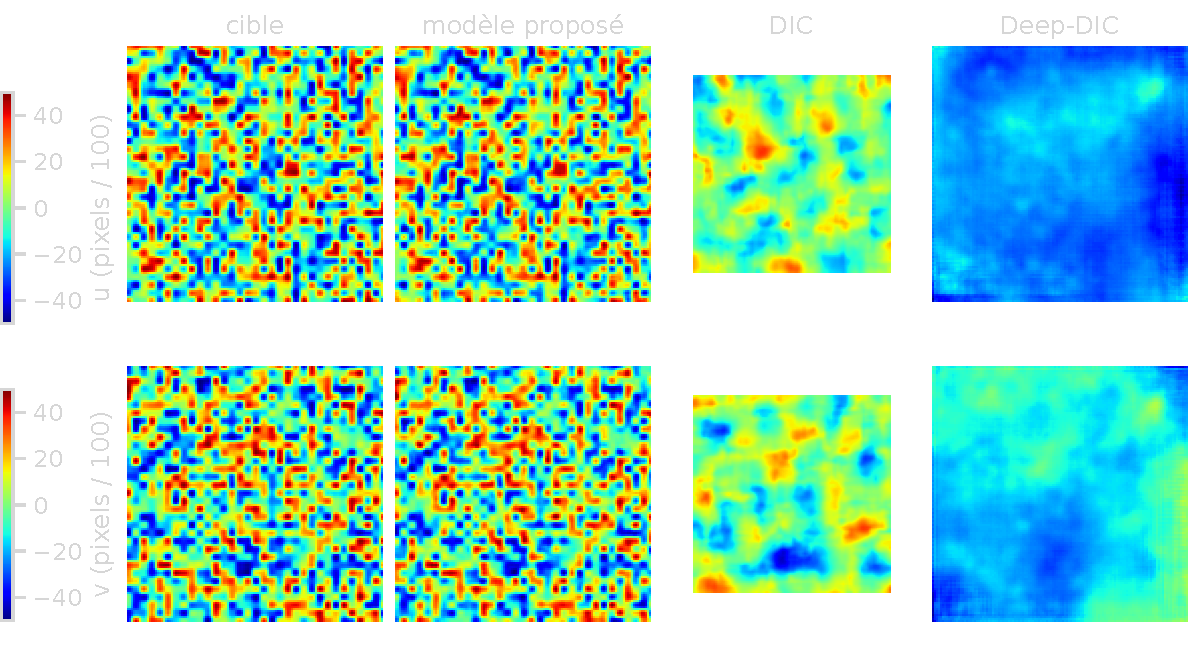
\includegraphics[width=90mm]{results/disp_5.pdf}} ;
			\node<2-3> at (0, 30mm) {Taille des éléments~: \alert{5 pixels}} ;
			
			\begin{scope}[xshift=0mm, yshift=-25mm]
				\node<3> at (-6mm, 0) {$\approx$ 95 ms} ;
				\node<3> at (14.5mm, 0) {$\approx$ 40 sec.} ;
				\node<3> at (35mm, 0) {$\approx$ 18 ms} ;
			\end{scope}

			\node<4> {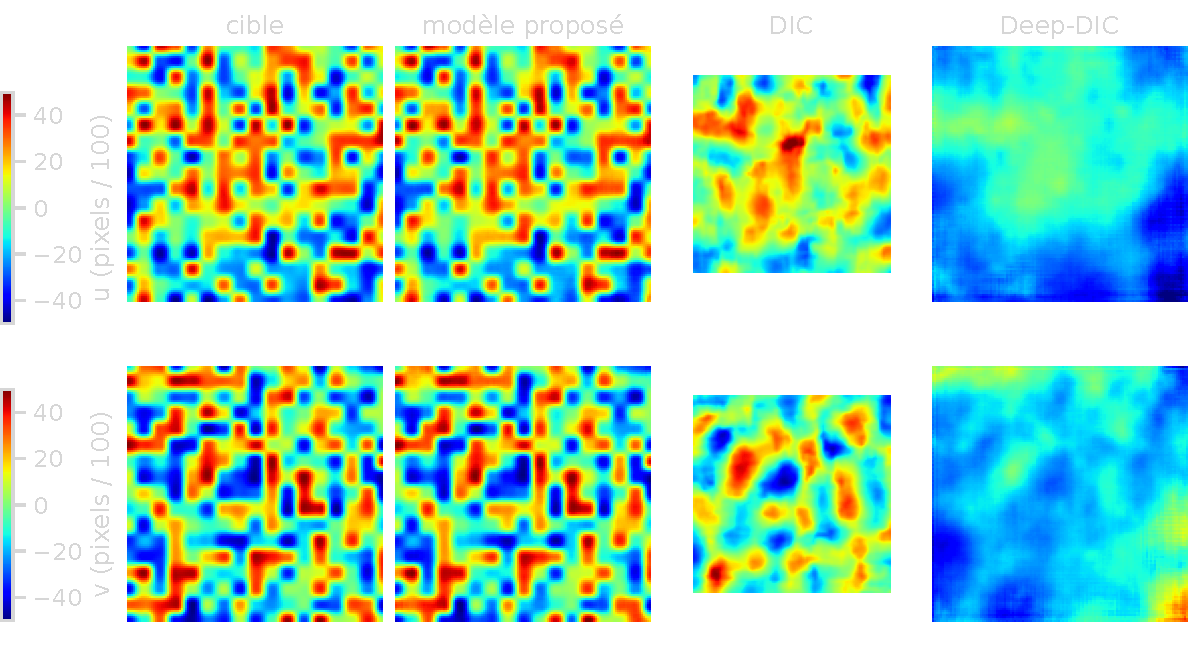
\includegraphics[width=90mm]{results/disp_9.pdf}} ;
			\node<4> at (0, 30mm) {Taille des éléments~: \alert{9 pixels}} ;
			
			\node<5-6> {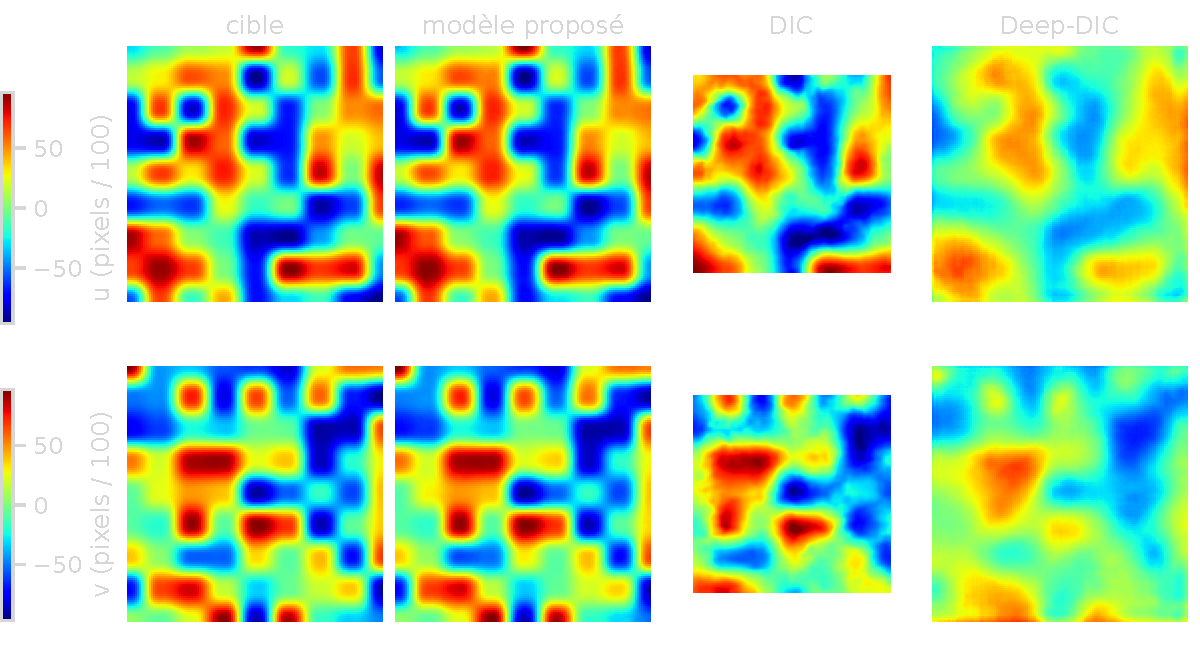
\includegraphics[width=90mm]{results/disp_17.pdf}} ;
			\node<5-6> at (0, 30mm) {Taille des éléments~: \alert{17 pixels}} ;
			\begin{scope}[xshift=0mm, yshift=-25mm]
				\node<6>[text centered, text width=30mm] at (14.5mm, 0) {\alert{Limite de\\résultion spatiale}} ;
			\end{scope}


			\node<7> {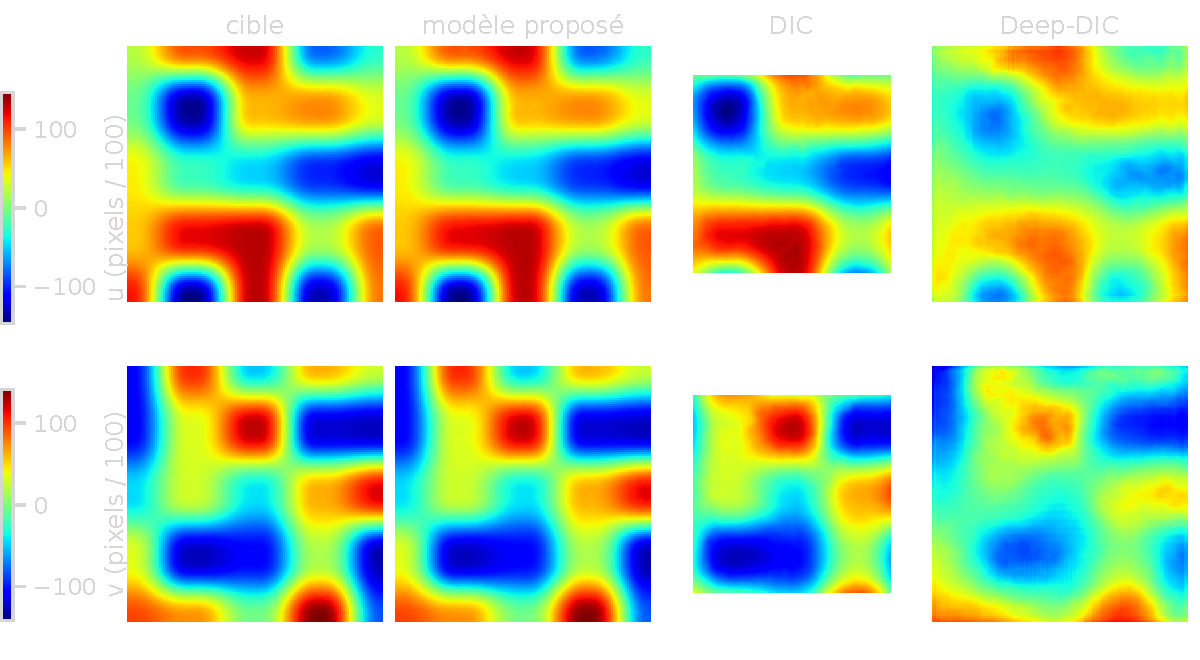
\includegraphics[width=90mm]{results/disp_33.pdf}} ;
			\node<7> at (0, 30mm) {Taille des éléments~: \alert{33 pixels}} ;
			
			\node<8> {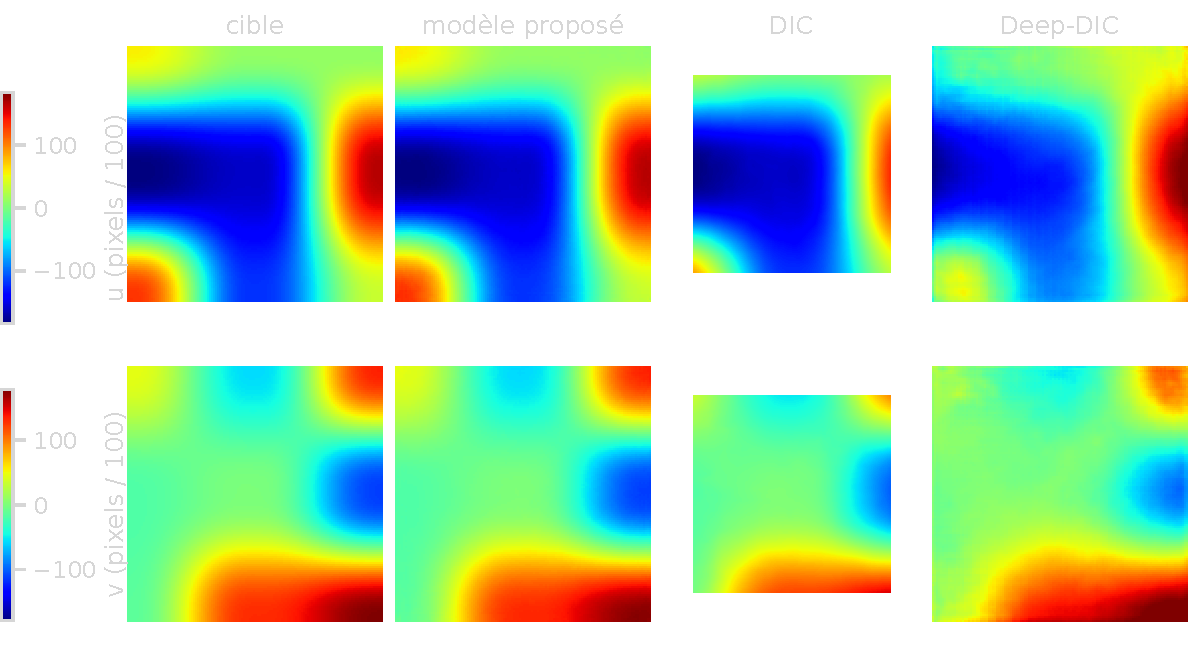
\includegraphics[width=90mm]{results/disp_65.pdf}} ;
			\node<8> at (0, 30mm) {Taille des éléments~: \alert{65 pixels}} ;

			\node<9> {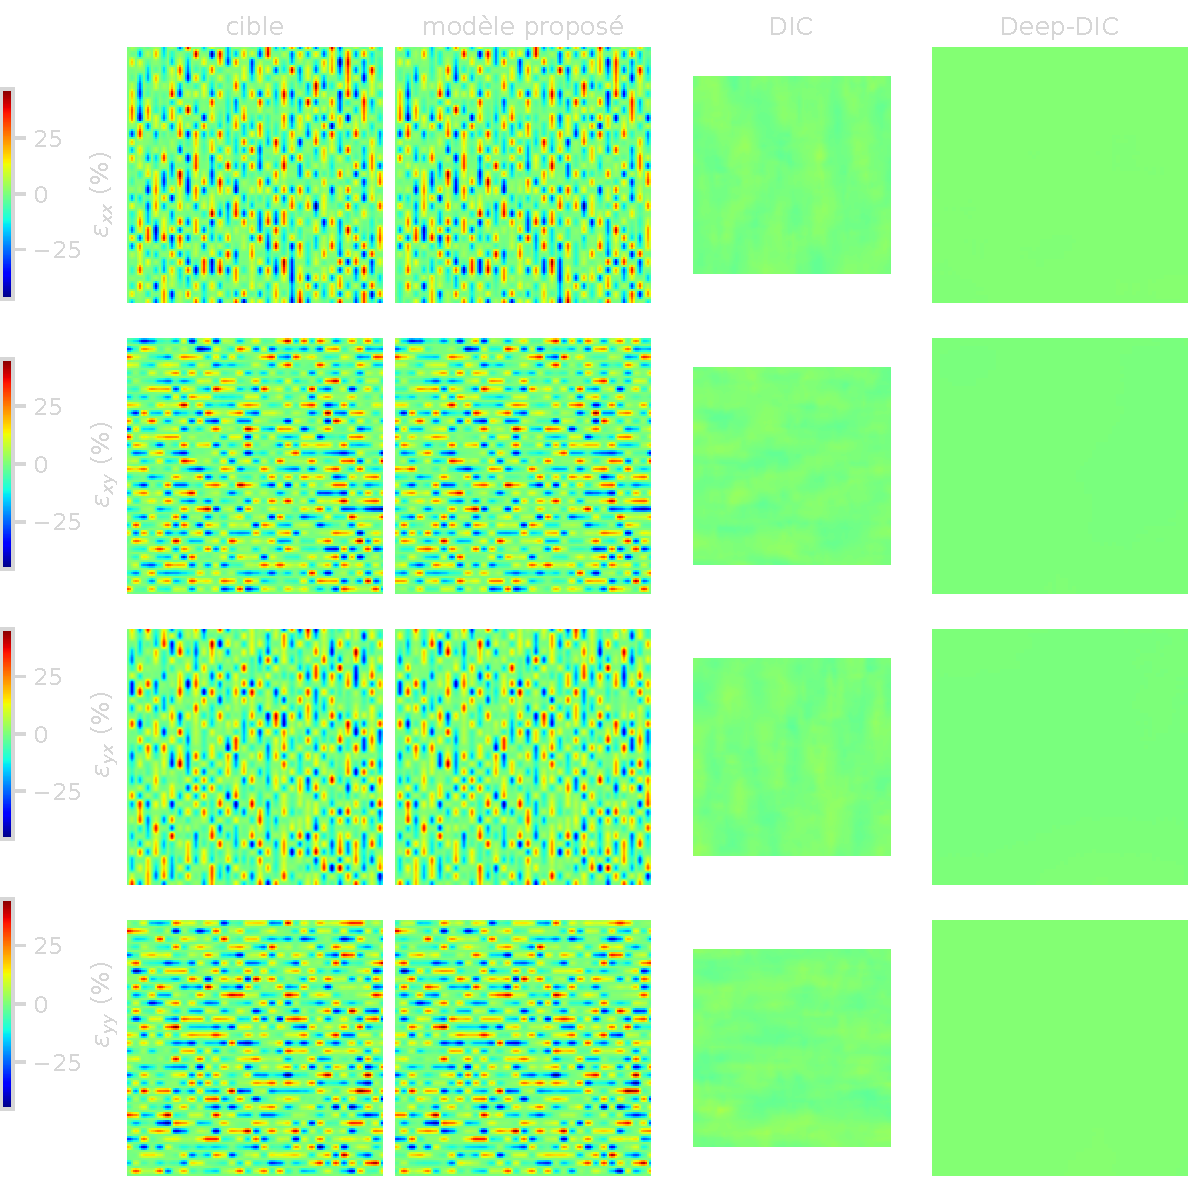
\includegraphics[width=70mm]{results/strain_5.pdf}} ;
			\node<9> at (0, 38mm) {Taille des éléments~: \alert{5 pixels}} ;

			\node<10> {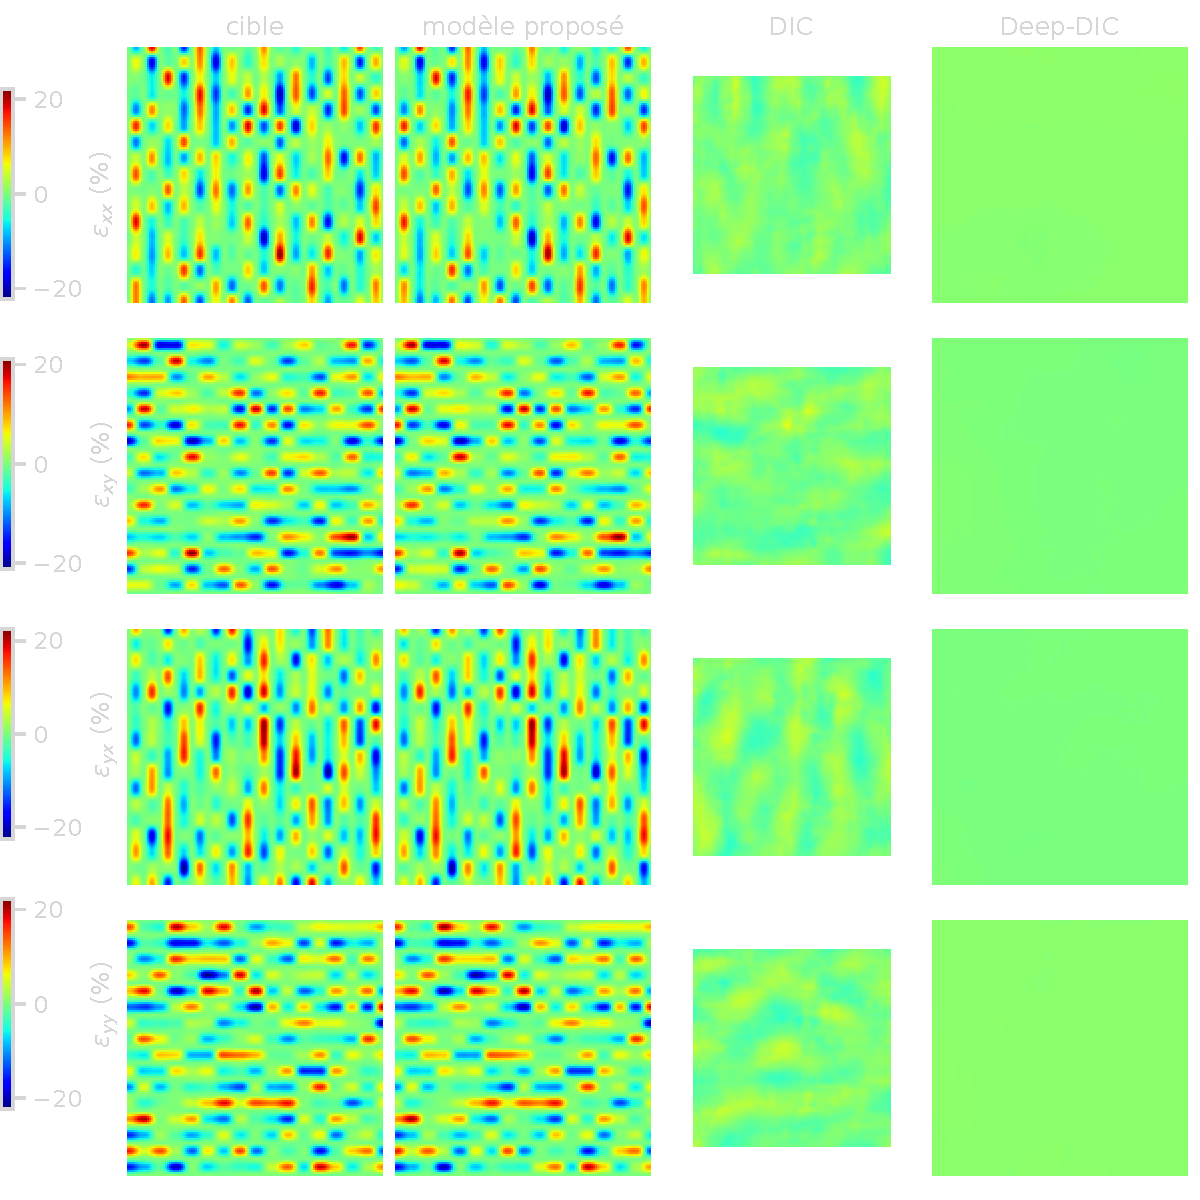
\includegraphics[width=70mm]{results/strain_9.pdf}} ;
			\node<10> at (0, 38mm) {Taille des éléments~: \alert{9 pixels}} ;

			\node<11> {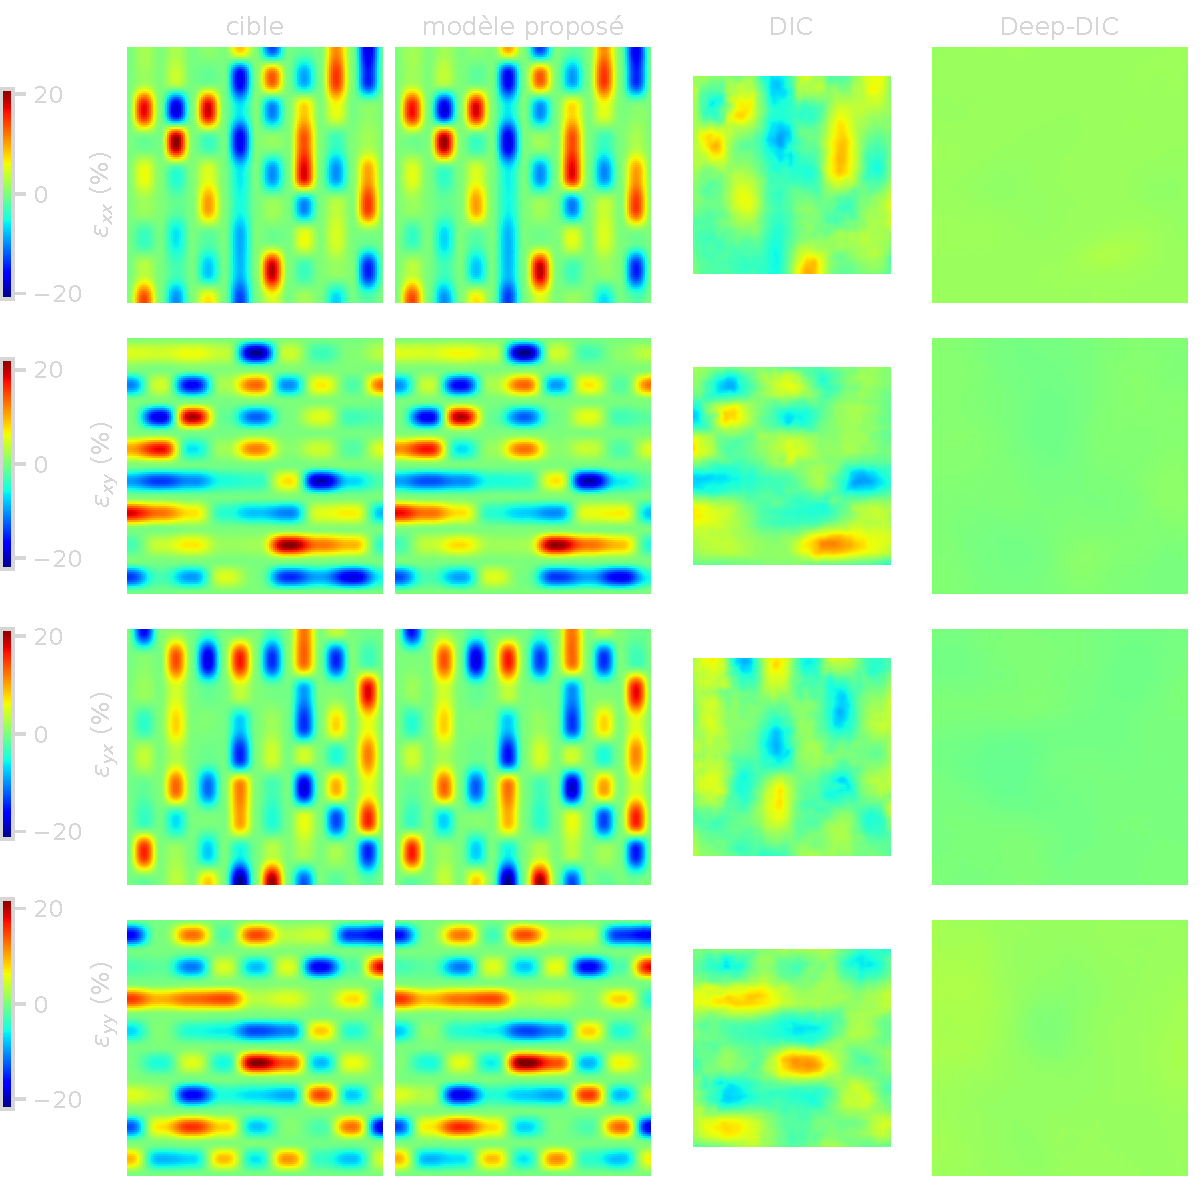
\includegraphics[width=70mm]{results/strain_17.pdf}} ;
			\node<11> at (0, 38mm) {Taille des éléments~: \alert{17 pixels}} ;

			\node<12> {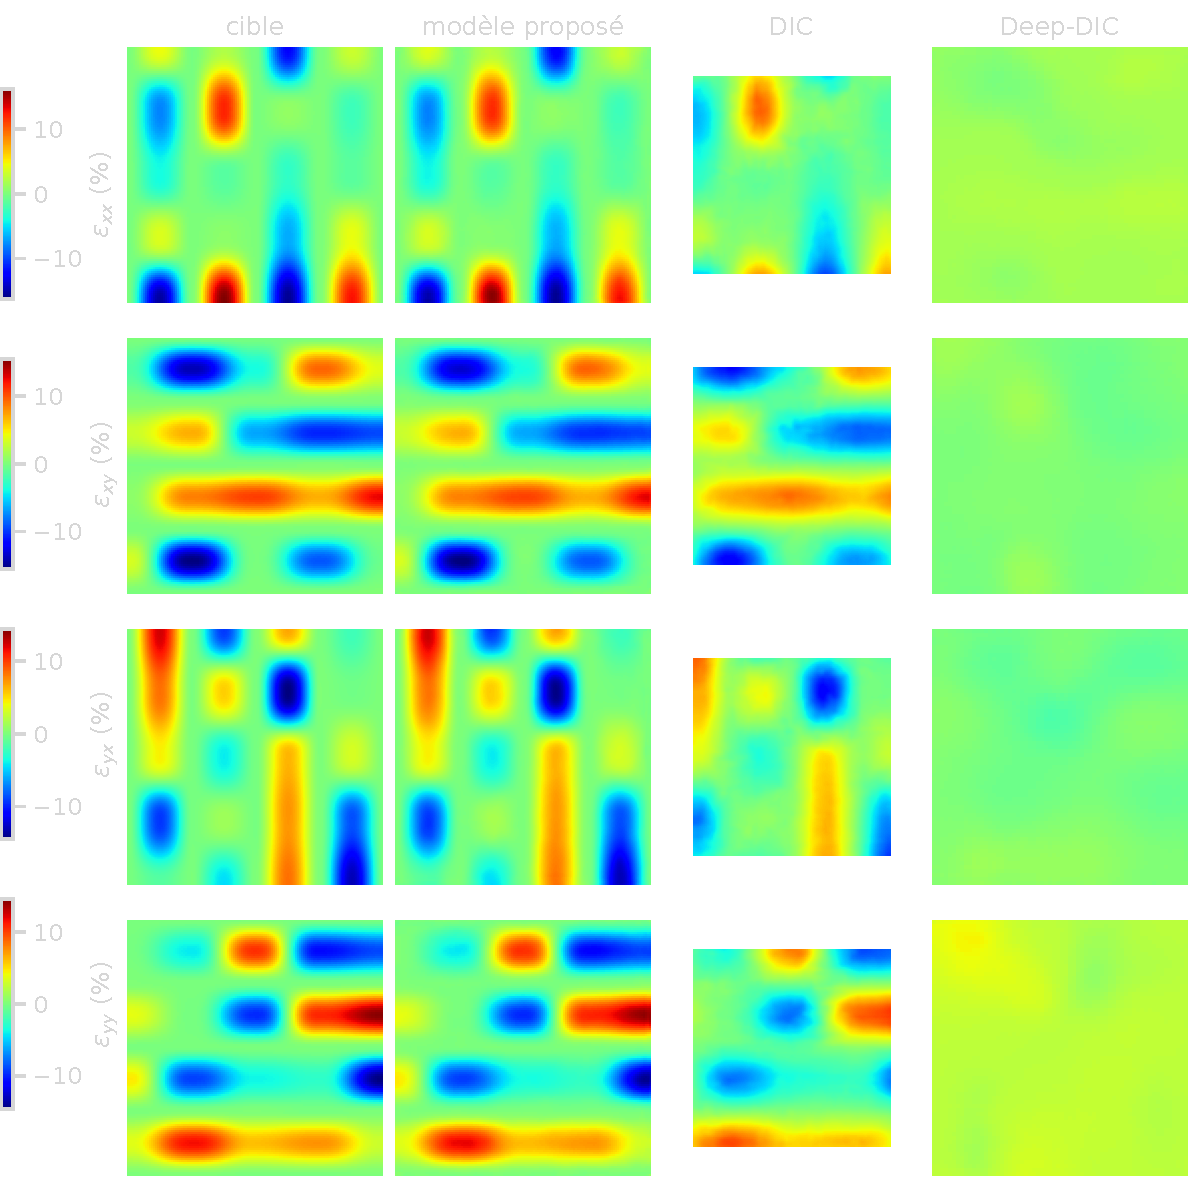
\includegraphics[width=70mm]{results/strain_33.pdf}} ;
			\node<12> at (0, 38mm) {Taille des éléments~: \alert{33 pixels}} ;

			\node<13> {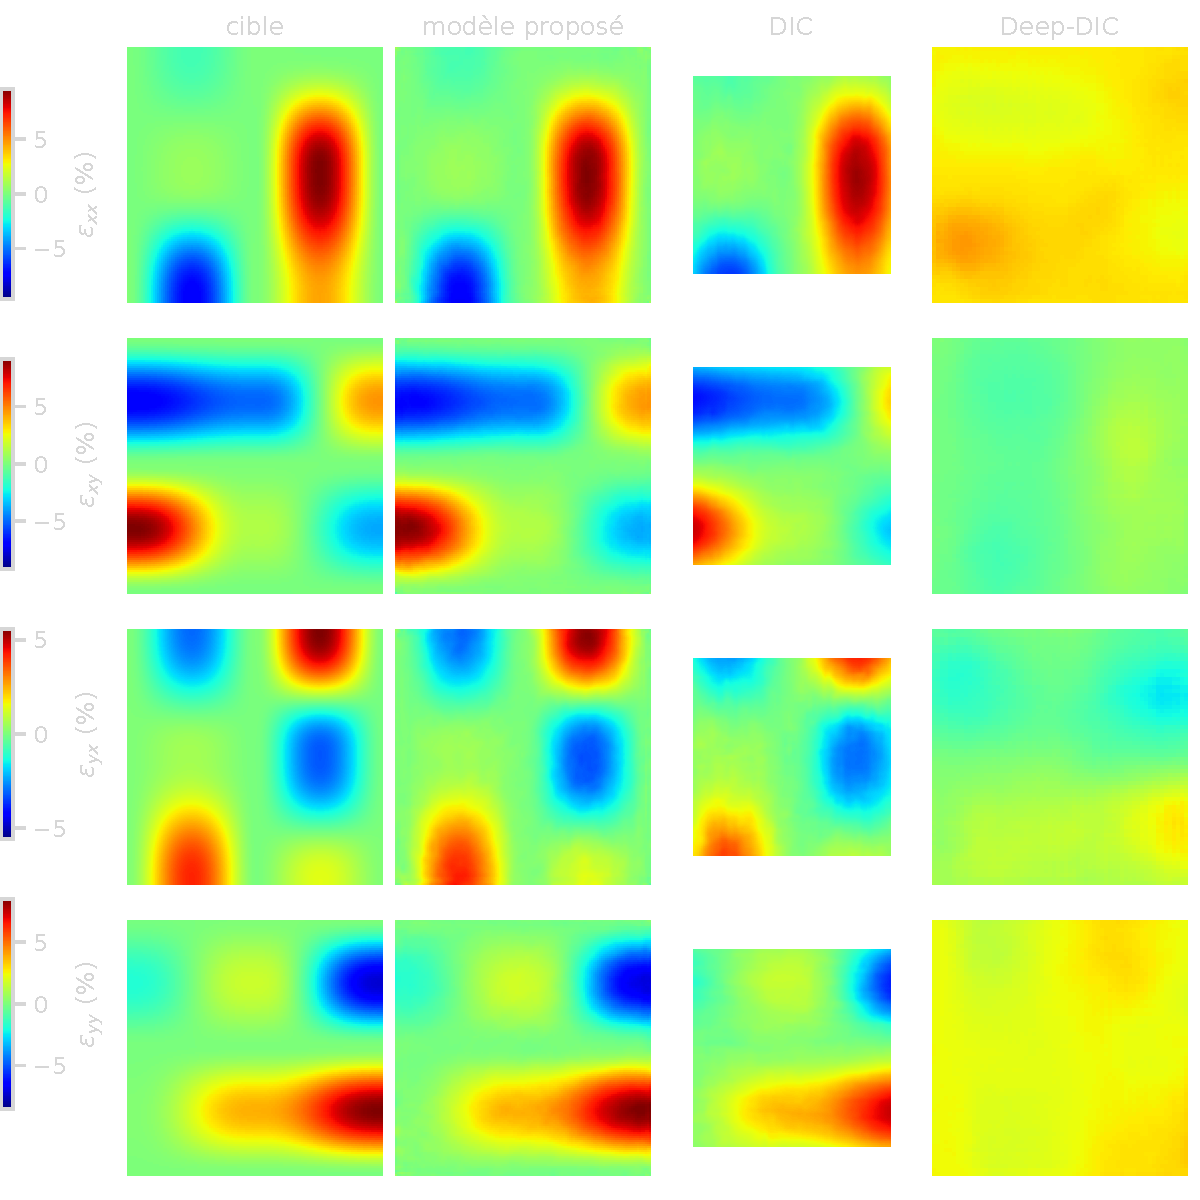
\includegraphics[width=70mm]{results/strain_65.pdf}} ;
			\node<13> at (0, 38mm) {Taille des éléments~: \alert{65 pixels}} ;
		\end{scope}
	\end{tikzpicture}
	\vfill
\end{frame}

\begin{frame}[t, label=ComparaisonMapsCcls]
	\vspace{0mm}
	\centering
	\vfill
	\begin{tikzpicture}
		\linespread{1}% <--- locally defined vertical line spacing in nodes
		\drawBorder
		\nodePageNumber

		\onlystyle<2->{shd1}{myShaded}
		\onlystyle<3->{shd2}{myShaded}
		\onlystyle<4->{shd3}{myShaded}
		\onlystyle<5->{shd4}{myShaded}
		\onlystyle<6->{shd5}{myShaded}
		% \onlystyle<7->{shd6}{myShaded}
		\node[shd1] at (\midX,80mm) {Comparaisons de modèles~: conclusions} ;

		\node<2->[box, shd2, text width=40mm] at (\midX-25mm,\midY+15mm) {Les modèles Deep Learning \alert{réduisent} le \alert{temps de calcul}} ;
		\node<3->[box, shd3, text width=40mm] at (\midX+25mm, \midY+15mm) {DIC~:\\calculs \alert{lents}\\limite spatiale \alert{17 / 35~pixels}} ;
		\node<4->[box, shd4, text width=40mm] (A) at (\midX-25mm, \midY-10mm) {Deep-DIC~:\\calculs \alert{rapides}\\limite spatiale \alert{33 / ?~pixels}} ;
		\node<5->[box, shd5, text width=40mm] (B) at (\midX+25mm, \midY-10mm) {Modèle proposé~:\\calculs \alert{rapides}\\\alert{bonne précision} pour le \alert{dataset}} ;
		\node<6->[box] (C) at (\midX, 12.5mm) {La \alert{limite spatiale} est liée au \alert{dataset d'entrainement}} ;
		\draw<6->[myarrow] (A) -- ++ (0, -13mm) -| ($(C.north) + (-15mm,0)$) ;
		\draw<6->[myarrow] (B) -- ++ (0, -13mm) -| ($(C.north) + (+15mm,0)$) ;
	\end{tikzpicture}
	\vfill
\end{frame}


\subsection{Images réelles}
\begin{frame}[t, label=PoutrePresentation]
	\vspace{0mm}
	\centering
	\vfill
	\begin{tikzpicture}
		\linespread{1}% <--- locally defined vertical line spacing in nodes
		\drawBorder
		\nodePageNumber

		\onlystyle<2->{shd1}{myShaded}
		% \onlystyle<3->{shd2}{myShaded}
		% \onlystyle<4->{shd3}{myShaded}
		% \onlystyle<5->{shd4}{myShaded}
		% \onlystyle<6->{shd5}{myShaded}
		% \onlystyle<7->{shd6}{myShaded}
		\node[shd1] at (\midX,80mm) {Séquence temporelle~: mesure de vibrations} ;

		\node at (\midX,\midY) {
			\includegraphics<2-4>[width=90mm]{poutre/image_poutre0.pdf}%
			\includegraphics<5>[width=90mm]{poutre/image_poutre1.pdf}%
			\includegraphics<6>[width=90mm]{poutre/image_poutre2.pdf}%
			\includegraphics<7>[width=90mm]{poutre/image_poutre3.pdf}%
			\includegraphics<8->[width=90mm]{poutre/image_poutre4.pdf}%
		} ;
		\node<3-> (A) at (\midX+35mm,\midY-25mm) {Encastrement} ;
		\draw<3->[myarrow]  ($(A.north) + (5mm, 0)$) -- (\midX+40mm, \midY) ;
		
		\node<4-> (B) at (\midX+10mm,\midY-22mm) {Marteau d'impact} ;
		\draw<4->[myarrow]  ($(B.north) + (0mm, 0)$) -- (\midX+29mm, \midY-2mm) ;
		
		\node<5->[text centered, text width=30mm] (C) at (\midX-22.5mm, \midY-27mm) {Motif \alert{différent} de ceux générés pour l'\alert{entrainement}} ;
		\draw<5->[myarrow]  ($(C.north) + (0mm, 0)$) -- (\midX-6mm, \midY-11mm) ;

		\node<9> at (\midX,10mm) {Suivi sur 20~000 images} ;
	\end{tikzpicture}
	\vfill
\end{frame}

\begin{frame}[t, label=PoutreResultats]
	\vspace{0mm}
	\centering
	\vfill
	\begin{tikzpicture}
		\linespread{1}% <--- locally defined vertical line spacing in nodes
		\drawBorder
		\nodePageNumber

		\onlystyle<2->{shd1}{myShaded}
		% \onlystyle<3->{shd2}{myShaded}
		% \onlystyle<4->{shd3}{myShaded}
		% \onlystyle<5->{shd4}{myShaded}
		% \onlystyle<6->{shd5}{myShaded}
		% \onlystyle<7->{shd6}{myShaded}
		\node[shd1] at (\midX,85mm) {Séquence temporelle~: résultats} ;

		\node<2-> at (\midX, \midY+15mm) {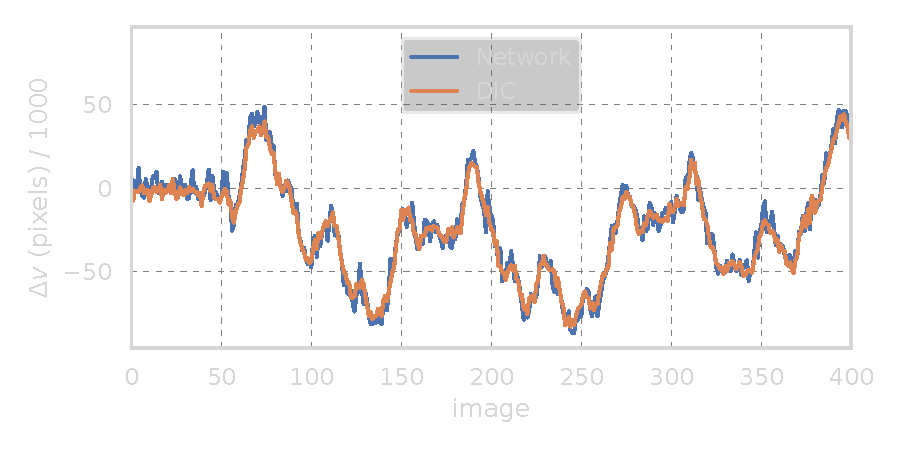
\includegraphics[width=80mm]{poutre/tracking_dv.pdf}} ;
		\node<3-> at (\midX, \midY-23mm) {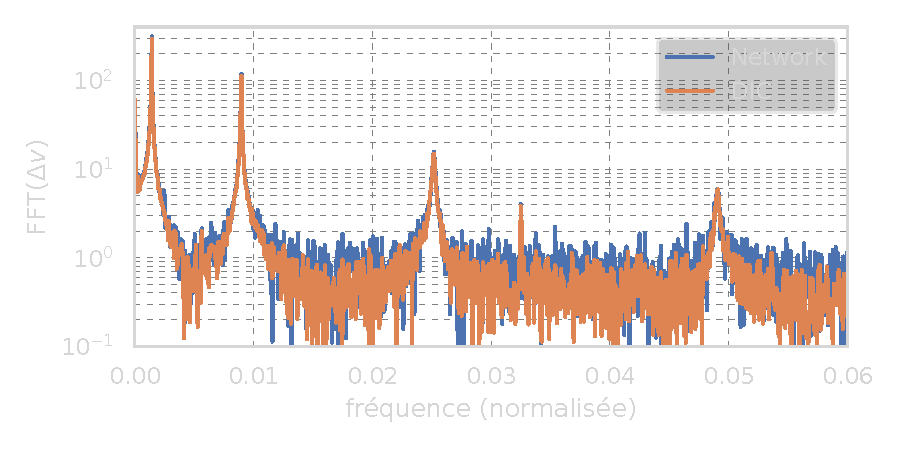
\includegraphics[width=80mm]{poutre/tracking_dv_fft.pdf}} ;

		\node<4->[text centered, text width=20mm] at (14mm,\midY-3mm) {\alert{Moins de bruit pour DIC}} ;
	\end{tikzpicture}
	\vfill
\end{frame}

\section{CONCLUSIONS}

\begin{frame}[t, label=CCLs]
	\vspace{0mm}
	\centering
	\vfill
	\begin{tikzpicture}
		\linespread{1}% <--- locally defined vertical line spacing in nodes
		\drawBorder
		\nodePageNumber

		\onlystyle<2->{shd1}{myShaded}
		\onlystyle<3->{shd2}{myShaded}
		\onlystyle<4->{shd3}{myShaded}
		\onlystyle<5->{shd4}{myShaded}
		\onlystyle<6->{shd5}{myShaded}
		% \onlystyle<7->{shd6}{myShaded}
		
		\node[box, shd1, text width=35mm] (A) at (\midX-25mm,\midY+25mm) {Les \alert{réseaux} de neurones \alert{convolutionnels} permettent d'\alert{accélérer} les \alert{traitements}} ;
		\node<2->[box, shd2, text width=35mm] (B) at (\midX+25mm,\midY+25mm) {L'\alert{optimisation} de l'architecture \alert{améliore} les \alert{résultats}} ;
		\node<3->[box, shd3, text width=35mm] (C) at (\midX-25mm,\midY+0mm) {Utiliser un \alert{dataset simulé} permet d'\alert{éviter} le \alert{sur-apprentissage}} ;
		\node<4->[box, shd4, text width=35mm] (D) at (\midX+25mm,\midY+0mm) {Mais \alert{nécessite} d'être suffisamment \alert{généraliste}} ;
		\node<5->[box, shd5, text width=35mm] (E) at (\midX-25mm,\midY-25mm) {La \alert{précision} obtenue est \alert{interessante}} ;
		\node<6->[box, text width=35mm] (F) at (\midX+25mm,\midY-25mm) {Limitation à des motifs \alert{suffisamment proches} de ceux du jeu d'\alert{entrainement}} ;

		\draw<2->[myarrow, shd2] (A) -- (B) ;
		% \draw<3->[myarrow] (B) -- (C) ;
		\draw<4->[myarrow, shd4] (C) -- (D) ;
		% \draw<5->[myarrow, shd5] (D) -- ++ (0, -12mm) -| (E) ;
		\draw<5->[myarrow, shd5] (C) -- (E) ;
		\draw<6->[myarrow] (E) -- (F) ;
	\end{tikzpicture}
	\vfill
\end{frame}

\section{PERSPECTIVES}
\begin{frame}[t, label=Perspectives]
	\vspace{0mm}
	\centering
	\vfill
	\begin{tikzpicture}
		\linespread{1}% <--- locally defined vertical line spacing in nodes
		\drawBorder
		\nodePageNumber

		\onlystyle<2->{shd1}{myShaded}
		\onlystyle<4->{shd2}{myShaded}
		% \onlystyle<5->{shd3}{myShaded}
		% \onlystyle<6->{shd4}{myShaded}
		% \onlystyle<7->{shd5}{myShaded}
		% \onlystyle<8->{shd6}{myShaded}

		\begin{scope}[xshift=\midX, yshift=\midY+15mm]
			\node[box, shd1, text width=35mm] (A) at (-25mm,0) {Besoin d'\alert{améliorer} le dataset} ;
			\node<2->[box, shd2, text width=35mm] (B) at (+25mm,+5mm) {Génération des motifs} ;
			\node<3->[box, shd2, text width=35mm] (B2) at (+25mm,-5mm) {Génération des valeurs cibles} ;
		\end{scope}

		\draw<2->[myarrow, shd2] (A.east) -- ++ (5mm, 0) |- (B) ;
		\draw<3->[myarrow, shd2] (A.east) -- ++ (5mm, 0) |- (B2) ;

		\begin{scope}[xshift=\midX, yshift=\midY-20mm]
			\node<4->[box, text width=35mm] (C) at (-25mm,0) {Exploration d'\alert{autres architectures}} ;
			\node<5->[box, text width=35mm] (D) at (25mm,0) {Utilisation de\\la méthode\\\alert{compound scaling}} ;
			\draw<5->[myarrow] (C) -- (D) ;
		\end{scope}
		% \node<4->[box, shd4, text width=35mm] (D) at (\midX+25mm,\midY+0mm) {Mais \alert{nécessite} d'être suffisamment \alert{généraliste}} ;
		% \node<5->[box, shd5, text width=35mm] (E) at (\midX-25mm,\midY-25mm) {La \alert{précision} obtenue est \alert{interessante}} ;
		% \node<6->[box, text width=35mm] (F) at (\midX+25mm,\midY-25mm) {Limitation à des motifs \alert{suffisamment proches} de ceux du jeu d'\alert{entrainement}} ;


	\end{tikzpicture}
	\vfill
\end{frame}


\begin{frame}[t, label=Merci]
	\vspace{0mm}
	\centering
	\vfill
	\begin{tikzpicture}
		\linespread{1}% <--- locally defined vertical line spacing in nodes
		\drawBorder
		\nodePageNumber

		\onlystyle<2->{shd1}{myShaded}
		% \onlystyle<3->{shd2}{myShaded}
		% \onlystyle<4->{shd3}{myShaded}
		% \onlystyle<5->{shd4}{myShaded}
		% \onlystyle<6->{shd5}{myShaded}
		% \onlystyle<7->{shd6}{myShaded}
		\node[shd1, text centered] at (\midX,\midY) {\Huge \alert{Merci} poutre votre \alert{attention}} ;

	\end{tikzpicture}
	\vfill
\end{frame}

\end{document}
